\documentclass[10pt,letterpaper]{article}
\usepackage[margin=1in]{geometry}
\usepackage{graphicx}
\usepackage{booktabs}
\usepackage{amsmath, amssymb}
\usepackage{hyperref}
\usepackage{caption}
\usepackage{subcaption}
\usepackage{xcolor}
\usepackage{multirow}
\usepackage{longtable}
\usepackage{tikz}
\usetikzlibrary{positioning,arrows.meta,shapes.geometric,fit,calc}
\usepackage{enumitem}

\hypersetup{colorlinks=true, linkcolor=blue, citecolor=blue}
\setlength{\parskip}{4pt}
\DeclareMathOperator*{\argmin}{arg\,min}
\DeclareMathOperator*{\argmax}{arg\,max}


\title{From SVMs to ResNets: \\ A Controlled Tier-Stratified Study of \\
Satellite Land-Use Classification on EuroSAT}
\author{Ekant Kapgate \and Saransh Soni \and Vineet Malewar \and Yashashav Devalapalli Kamalraj \\
\small{San Jos\'{e} State University --- CMPE 257: Machine Learning}}
\date{\today}

\begin{document}
\maketitle

\section*{Code Repository}
Public Git repository (code, results, figures, and report sources): \url{https://github.com/yashashav-dk/cmpe257-eurosat}

\begin{abstract}
We present a controlled, tier-stratified study of land-use classification on EuroSAT RGB (10 classes, 27{,}000 64$\times$64 Sentinel-2 patches). Four model tiers are compared on an identical seed-42 stratified 70/15/15 split: (T1) classical linear and kernel models on PCA-reduced raw pixels; (T2) classical models on a 1{,}860-D handcrafted-feature vector (HOG + per-channel color histograms); (T3) a 391K-parameter shallow CNN with optimizer and regularization ablations; and (T4) a fine-tuned ImageNet-pretrained ResNet-18. Test accuracy improves monotonically across tiers from 0.6872 (T1, SVM-RBF on PCA(500)) to 0.8309 (T2, SVM-RBF on HOG+color), 0.9657 (T3, ShallowCNN+BatchNorm), and 0.9816 $\pm$ 0.0016 (T4, ResNet-18, 3 seeds). Two systematic ablations on the shallow CNN ground the higher-tier choices: a $6 \times 3 \times 3$ optimizer ablation (\textbf{54 runs}, 100 epochs each) shows the top four optimizers (Adam, NAG, SGD+Momentum, RMSProp) tie within 0.3pp at their best learning rates while Adam reaches 90\% validation accuracy in 10 epochs versus 13--21 for the rest; a $9 \times 3$ regularization ablation (\textbf{27 runs}) shows BatchNorm alone yields the largest single-technique improvement (+1.1pp over baseline), while combining all five techniques actually \emph{hurts} (\hbox{$-3$pp}) through over-regularization. Paired $t$-tests at $\alpha{=}0.05$ confirm the ResNet-18 vs.\ ShallowCNN+BN gap ($p{=}0.011$) is statistically significant; the +BN vs.\ baseline gap ($p{=}0.072$) is marginal at three seeds. Per-class analysis identifies four spectrally-similar crop classes (PermanentCrop, AnnualCrop, HerbaceousVegetation, Pasture) as the consistent bottleneck across all tiers. We release all code, run logs, predictions, and figures publicly.
\end{abstract}

\tableofcontents
\newpage

\section{Introduction}

\subsection{Motivation}
Optical Earth Observation programs --- principally the European Space Agency's Sentinel-2 mission and NASA's Landsat constellation --- generate petabytes of multispectral imagery every year. Translating that imagery into useful information products (urban-extent maps, deforestation alerts, crop-type inventories, disaster-impact assessments) requires reliable land-use classification at scale. Manual annotation does not scale to global coverage; supervised machine learning is the only practical route.

The EuroSAT benchmark introduced by Helber et al.~\cite{helber2019} has become one of the de facto reference points for evaluating land-use classifiers on Sentinel-2 imagery. It provides 27{,}000 labeled $64\times64$ patches drawn from across Europe and split into 10 classes: AnnualCrop, Forest, HerbaceousVegetation, Highway, Industrial, Pasture, PermanentCrop, Residential, River, and SeaLake. While the original work reported a 98.57\% accuracy with a fine-tuned ResNet-50 on the multispectral version, the public RGB subset (used in this study) admits a wide range of model choices --- from raw-pixel logistic regression to deep transfer learning --- which makes it an ideal venue for a controlled comparative study of how each modeling decision contributes to the final classifier.

\subsection{Why a Tiered Comparison?}
Most published EuroSAT results are point comparisons: a single architecture, a single training recipe, a single seed. Such reports are useful but make it hard to attribute the source of each improvement. Did transfer learning help more than the architecture itself? Did data augmentation matter more than the optimizer? Without a controlled hierarchy, these questions remain anecdotal.

This study is built around a four-tier hierarchy designed so that each tier strictly subsumes the prior tier in expressive capacity. The intended reading: an improvement at tier $k+1$ over tier $k$ is the contribution of the additional capacity introduced at that step (handcrafted feature engineering, learned features, transfer learning), holding the data, the split, and the evaluation protocol fixed.

\subsection{Research Questions and Contributions}
We formalize the study around three research questions:
\begin{itemize}[leftmargin=2em]
    \item \textbf{RQ1.} How does test accuracy scale across the tier hierarchy (raw pixels $\rightarrow$ handcrafted features $\rightarrow$ shallow learned features $\rightarrow$ deep transfer)? At which tier does the marginal return diminish?
    \item \textbf{RQ2.} Among six widely-used optimizers (SGD, SGD+Momentum, NAG, Adam, Adagrad, RMSProp), which converges fastest and which generalizes best on the shallow CNN? Does the dataset confirm the SGD-with-momentum-dominates-Adam claim of Wilson et al.~\cite{wilson2017}?
    \item \textbf{RQ3.} Among five regularization techniques (L2, Dropout, BatchNorm, DataAugmentation, EarlyStopping), which most reduces the train/test overfitting gap on the shallow CNN, and how do they compose when stacked?
\end{itemize}

We summarize our contributions as follows:
\begin{itemize}[leftmargin=2em]
    \item A reproducible four-tier benchmark on EuroSAT RGB with a single fixed seed-42 stratified 70/15/15 split. Test set is touched exactly once per model.
    \item A 54-run optimizer ablation (Experiment B) on the shallow CNN baseline with multi-seed variance reporting and convergence-speed analysis.
    \item A 27-run regularization ablation (Experiment C) demonstrating an over-regularization phenomenon: stacking all five techniques degrades accuracy by 3pp versus the best single technique.
    \item A 3-seed ResNet-18 fine-tuning result (mean acc 0.9816 $\pm$ 0.0016) along with paired-$t$-test significance comparisons against shallow-CNN variants.
    \item A per-class analysis across 8 representative models identifying the four-way crop confusion that bottlenecks every tier.
    \item A 100$\times$ training speedup on the shallow CNN (1.06 s/epoch vs.\ 105 s/epoch) by replacing the standard Drive-backed PyTorch \texttt{ImageFolder} loader with a GPU-resident \texttt{TensorDataset} --- without which the 54-run optimizer ablation would have required 158 hours of A100 time.
    \item A fully open release: code, run logs, predictions, all figures, and the LaTeX source of this report on GitHub.
\end{itemize}

\subsection{Paper Organization}
Section~\ref{sec:problem} formalizes the classification problem and lists scope boundaries. Section~\ref{sec:related} surveys related work in EO benchmarks, classical and deep models, transfer learning, optimization, and regularization. Section~\ref{sec:solution} describes the tier hierarchy and the building blocks. Section~\ref{sec:experiments} enumerates the five experiments. Section~\ref{sec:setup} gives the full experimental protocol. Section~\ref{sec:results} reports tier-by-tier results, the optimizer and regularization ablations, the final comparison, statistical tests, and per-class analysis. Section~\ref{sec:discussion} interprets the findings against prior work. Sections~\ref{sec:limitations}--\ref{sec:future} discuss limitations and future directions, and Section~\ref{sec:conclusions} concludes. Section~\ref{sec:contributions} documents per-member contributions. Appendices contain full hyperparameter tables, full per-run results for Experiments B and C, expanded per-class metrics, all confusion matrices, and a NeurIPS-style reproducibility checklist.

\section{Problem Statement}
\label{sec:problem}

\subsection{Formal Setting}
Let $\mathcal{X} \subset \mathbb{R}^{H \times W \times 3}$ denote the input space of EuroSAT RGB patches with $H{=}W{=}64$, and let $\mathcal{Y} = \{1, 2, \ldots, 10\}$ index the ten land-use classes. The data is drawn i.i.d.\ from an unknown joint distribution $\mathcal{D}$ over $\mathcal{X} \times \mathcal{Y}$. We seek a classifier $f_\theta : \mathcal{X} \rightarrow \Delta^{10}$, parametrized by $\theta$, that minimizes the expected cross-entropy loss:
\begin{equation}
\theta^\ast = \argmin_\theta \mathbb{E}_{(\mathbf{x}, y) \sim \mathcal{D}} \left[ -\log f_\theta(\mathbf{x})_y \right].
\end{equation}
We approximate the expectation with the empirical risk on the training split $S_\text{tr}$:
\begin{equation}
\hat{\theta} = \argmin_\theta \frac{1}{|S_\text{tr}|} \sum_{(\mathbf{x}, y) \in S_\text{tr}} \big( -\log f_\theta(\mathbf{x})_y \big) + \lambda \, \Omega(\theta),
\end{equation}
where $\Omega(\theta)$ is an optional regularizer (e.g., $\ell_2$ weight decay, dropout-induced stochasticity) and $\lambda$ controls its strength. The classifier is evaluated by argmax-accuracy on the held-out test split $S_\text{te}$:
\begin{equation}
\text{Acc}(\hat{\theta}; S_\text{te}) = \frac{1}{|S_\text{te}|} \sum_{(\mathbf{x}, y) \in S_\text{te}} \mathbb{1}\!\left[ \argmax_{y'} f_{\hat\theta}(\mathbf{x})_{y'} = y \right].
\end{equation}

\subsection{Sub-Problems}
The classifier $f_\theta$ decomposes into a feature extractor $\phi : \mathcal{X} \rightarrow \mathcal{Z}$ followed by a classifier head $g : \mathcal{Z} \rightarrow \Delta^{10}$, so $f_\theta = g_\theta \circ \phi$. The four tiers of this study correspond to four choices of $\phi$:
\begin{itemize}[leftmargin=2em]
    \item $\phi_\text{T1}$: PCA projection of vectorized pixel intensities (deterministic, parameter-free except for the projection matrix learned on the training set).
    \item $\phi_\text{T2}$: HOG descriptor concatenated with per-channel color histograms (deterministic, hand-engineered).
    \item $\phi_\text{T3}$: a small convolutional encoder learned end-to-end with $g$.
    \item $\phi_\text{T4}$: an ImageNet-pretrained convolutional encoder fine-tuned end-to-end with $g$.
\end{itemize}
Within $\phi_\text{T3}$, two sub-questions arise: which optimizer best estimates $\hat\theta$ from the training data (RQ2), and which regularizer $\Omega$ best controls the train/test gap (RQ3).

\subsection{Hypotheses (a priori)}
Before running any experiment, we recorded three testable hypotheses:
\begin{enumerate}[leftmargin=2em]
    \item \textbf{H1.} Test accuracy will be monotonic in tier index: $\text{Acc}_\text{T1} < \text{Acc}_\text{T2} < \text{Acc}_\text{T3} < \text{Acc}_\text{T4}$, with the largest jump at T2$\rightarrow$T3 (handcrafted $\rightarrow$ learned features).
    \item \textbf{H2.} Adam will converge fastest but SGD+Momentum will achieve the best final accuracy, consistent with Wilson et al.~\cite{wilson2017}.
    \item \textbf{H3.} Combining all five regularization techniques will yield the highest accuracy among Experiment C configurations.
\end{enumerate}
Section~\ref{sec:results} reports outcomes against each hypothesis.

\subsection{Scope and Boundaries}
The following are deliberately out of scope:
\begin{itemize}[leftmargin=2em]
    \item \emph{Multispectral inputs.} EuroSAT also provides 13 Sentinel-2 bands (visible + NIR + SWIR + atmospheric); we use only the RGB subset to keep all four tiers compatible with standard ImageNet-pretrained backbones.
    \item \emph{Architecture search.} We fix one architecture per tier and study the effect of optimization and regularization, not architectural variation.
    \item \emph{Cross-distribution evaluation.} EuroSAT is geographically European; cross-continent transfer (e.g.\ to RESISC45 \cite{cheng2017}) is left to future work.
    \item \emph{Semantic segmentation.} EuroSAT is a patch-classification benchmark; pixel-level segmentation is a distinct task.
    \item \emph{Adversarial robustness and fairness.} Out of scope for a baseline accuracy study.
\end{itemize}

\subsection{Why a Tiered Experimental Design?}
The tiered design isolates the contribution of each modeling decision. Because data, splits, evaluation metric, and seeds are held constant across tiers, any monotonic gain in accuracy from tier $k$ to tier $k{+}1$ is directly attributable to the additional modeling capacity introduced at that step, not to confounders such as different preprocessing or different test sets. The two ablations within Tier 3 (Exp B and Exp C) further isolate optimization-quality and regularization-strength effects from architectural effects.

\section{Related Work}
\label{sec:related}

\subsection{EuroSAT and Earth-Observation Benchmarks}
Helber et al.~\cite{helber2019} introduced EuroSAT in 2019 as a 27{,}000-image, 10-class land-use benchmark drawn from Sentinel-2 tiles over Europe. Their reference numbers (98.57\% with ResNet-50 multispectral, 98.33\% RGB) established the strong-supervised ceiling. EuroSAT has since been used as a standard benchmark in transfer-learning surveys, few-shot remote-sensing studies, and self-supervised pretraining work. Cheng et al.~\cite{cheng2017} surveyed remote-sensing scene classification more broadly and introduced RESISC45, a 45-class higher-resolution alternative; Sumbul et al.~\cite{bigearthnet2019} introduced BigEarthNet, a multi-label benchmark of 590{,}326 patches that better reflects real-world EO scale. Stivaktakis et al.~\cite{stivaktakis2019} and Pelletier et al.~\cite{pelletier2019} studied temporal extensions of EuroSAT-style classification.

\subsection{Handcrafted Visual Features}
Before deep learning, computer vision relied on hand-engineered descriptors. Histogram of Oriented Gradients, introduced by Dalal and Triggs~\cite{dalal2005} for pedestrian detection, captures local edge orientation distributions and remains a strong baseline on textured imagery. Lowe's SIFT~\cite{lowe2004} and Bay et al.'s SURF~\cite{bay2008} provide scale- and rotation-invariant keypoint descriptors; Local Binary Patterns (Ojala et al.~\cite{ojala2002}) capture micro-texture. For land-use classification specifically, Yang and Newsam~\cite{yang2010} compared SIFT-bag-of-words with color histograms on the UC-Merced dataset. Color histograms (Swain and Ballard~\cite{swain1991}) remain a simple but effective complement to gradient-based descriptors: they capture chromatic information that gradient histograms discard. The 1{,}860-D HOG-plus-color feature vector used at Tier 2 of this study follows this combined-descriptor tradition.

\subsection{Classical Machine Learning on Imagery}
Logistic regression, support vector machines, and kernel methods have been applied to imagery via dimensionality-reduced or hand-engineered features. Turk and Pentland's Eigenfaces~\cite{turk1991} demonstrated that PCA-projected pixel intensities support viable face recognition; Boutell et al.~\cite{boutell2004} applied SVMs to multi-label scene classification. Cortes and Vapnik's original SVM~\cite{cortes1995} and the kernel trick (Sch\"{o}lkopf and Smola~\cite{scholkopf2002}) provide the theoretical basis for the RBF-SVC variants used at Tier 1 and Tier 2. The cuML library (NVIDIA RAPIDS~\cite{rapids2018}) provides GPU-accelerated implementations of these classical estimators that are critical for our 80-fit grid search at Tier 1.

\subsection{Deep Convolutional Networks}
Krizhevsky et al.~\cite{alexnet2012} demonstrated that deep CNNs trained with backpropagation and GPUs could decisively outperform classical pipelines on ImageNet, kicking off the modern era of computer vision. Architectural follow-ups include VGG (Simonyan and Zisserman~\cite{vgg2014}), GoogLeNet/Inception (Szegedy et al.~\cite{googlenet2015}), and especially ResNet (He et al.~\cite{he2016}), whose residual connections enabled training of much deeper networks and remain a workhorse for transfer learning. Our Tier 4 uses ResNet-18, the smallest member of the ResNet family. EfficientNet (Tan and Le~\cite{efficientnet2019}) and Vision Transformers (Dosovitskiy et al.~\cite{vit2020}) represent more recent architectural directions that we leave to future work.

\subsection{Transfer Learning}
Yosinski et al.~\cite{yosinski2014} characterized the transferability of features in deep networks, showing that earlier layers transfer more readily than task-specific later layers. Pan and Yang~\cite{pan2010} surveyed transfer learning more broadly. The dominant practical recipe --- pretrain on ImageNet, replace the final classifier, fine-tune end-to-end --- has been validated repeatedly on remote-sensing data, including by Helber et al.\ themselves~\cite{helber2019}. Recent work in self-supervised pretraining (SimCLR by Chen et al.~\cite{simclr2020}, DINO by Caron et al.~\cite{dino2021}, MAE by He et al.~\cite{mae2021}) offers an alternative source of pretrained weights that does not require ImageNet labels but is out of scope here.

\subsection{Optimization for Deep Learning}
Stochastic gradient descent in its modern minibatch form dates back at least to Bottou~\cite{bottou1998}. Polyak's momentum~\cite{polyak1964} and Nesterov's accelerated gradient~\cite{nesterov1983} predate deep learning but became standard tools after LeCun et al.~\cite{lecun1998} and others. Duchi et al.\ introduced Adagrad~\cite{adagrad2011}; RMSProp was popularized in Hinton's lecture notes. Kingma and Ba~\cite{kingma2014} introduced Adam, combining momentum with adaptive per-parameter learning rates. Wilson et al.~\cite{wilson2017} argued that adaptive methods generalize worse than well-tuned SGD with momentum, sparking a long debate. Choi et al.~\cite{choi2019} countered that conclusions depend heavily on the hyperparameter tuning budget; Schmidt et al.~\cite{schmidt2021} performed a 50-thousand-run benchmark and found that no single optimizer dominates across tasks. Loshchilov and Hutter~\cite{loshchilov2019} introduced AdamW, decoupling weight decay from the gradient update. Our Experiment B is a small-scale instance of this comparison restricted to a fixed shallow CNN on EuroSAT.

\subsection{Regularization}
Krogh and Hertz~\cite{krogh1992} provided the early theoretical analysis of $\ell_2$ weight decay in neural networks. Srivastava et al.~\cite{dropout2014} introduced Dropout. Ioffe and Szegedy~\cite{batchnorm2015} introduced Batch Normalization, originally framed as reducing internal covariate shift; subsequent work (Santurkar et al.~\cite{santurkar2018}, Bjorck et al.~\cite{bjorck2018}) reframed its effect in terms of optimization-landscape smoothing. Early stopping has a long history in statistics; Prechelt~\cite{prechelt1998} provided practical patience heuristics. Data augmentation in the deep-learning era was systematized by Krizhevsky et al.~\cite{alexnet2012}; recent extensions include Mixup (Zhang et al.~\cite{mixup2018}), CutMix (Yun et al.~\cite{cutmix2019}), RandAugment (Cubuk et al.~\cite{randaugment2020}), and AugMix (Hendrycks et al.~\cite{augmix2020}). Our Experiment C tests classical augmentation (flips + rotations + color jitter) but leaves these stronger schemes for future work.

\section{Solution}
\label{sec:solution}

\subsection{Tier Hierarchy}
The classifier $f = g \circ \phi$ admits four feature-extractor choices, ordered by capacity. Figure~\ref{fig:pipeline} sketches the experimental pipeline.

\begin{figure}[h]
\centering
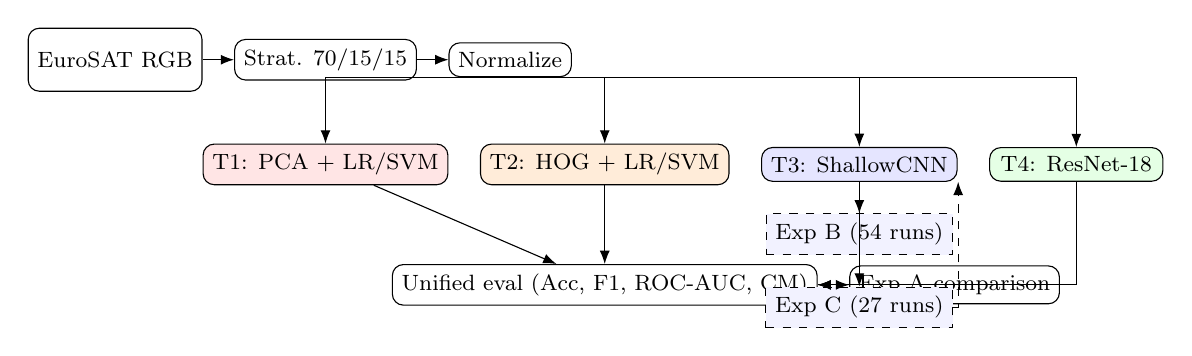
\begin{tikzpicture}[node distance=4mm, every node/.style={font=\footnotesize}]
\node[draw, rounded corners, minimum width=15mm, minimum height=8mm] (data) {EuroSAT RGB};
\node[draw, rounded corners, right=of data, minimum width=18mm] (split) {Strat. 70/15/15};
\node[draw, rounded corners, right=of split, minimum width=14mm] (norm) {Normalize};
\node[draw, fill=red!10, rounded corners, below=8mm of split, minimum width=20mm] (t1) {T1: PCA + LR/SVM};
\node[draw, fill=orange!15, rounded corners, right=of t1, minimum width=22mm] (t2) {T2: HOG + LR/SVM};
\node[draw, fill=blue!10, rounded corners, right=of t2, minimum width=22mm] (t3) {T3: ShallowCNN};
\node[draw, fill=green!10, rounded corners, right=of t3, minimum width=22mm] (t4) {T4: ResNet-18};
\node[draw, rounded corners, below=10mm of t2, minimum width=24mm] (eval) {Unified eval (Acc, F1, ROC-AUC, CM)};
\node[draw, rounded corners, right=of eval, minimum width=22mm] (compare) {Exp A comparison};
\node[draw, dashed, below=4mm of t3, minimum width=22mm, fill=blue!5] (expb) {Exp B (54 runs)};
\node[draw, dashed, below=4mm of expb, minimum width=22mm, fill=blue!5] (expc) {Exp C (27 runs)};
\draw[-Latex] (data) -- (split); \draw[-Latex] (split) -- (norm);
\draw[-Latex] (norm.south) -| (t1.north);
\draw[-Latex] (norm.south) -| (t2.north);
\draw[-Latex] (norm.south) -| (t3.north);
\draw[-Latex] (norm.south) -| (t4.north);
\draw[-Latex] (t1) -- (eval); \draw[-Latex] (t2) -- (eval);
\draw[-Latex] (t3) |- (eval); \draw[-Latex] (t4) |- (eval);
\draw[-Latex, dashed] (t3) -- (expb); \draw[-Latex, dashed] (expb) -- (expc);
\draw[-Latex, dashed] (expc.east) -| ([xshift=-15mm]t4.south);
\draw[-Latex] (eval) -- (compare);
\end{tikzpicture}
\caption{Experimental pipeline. Solid arrows show data flow; dashed arrows show ablation studies that feed hyperparameter choices forward (Exp B fixes the optimizer for Exp C; Exp C confirms regularization choices used at Tier 4).}
\label{fig:pipeline}
\end{figure}

\subsection{Tier 1 --- PCA + Classical}
Each $64{\times}64{\times}3$ image is vectorized to $\mathbf{x} \in \mathbb{R}^{12288}$. A standard scaler centers and unit-variances each pixel coordinate using statistics from the training split. Principal Component Analysis projects the standardized vector onto the top-$k$ eigenvectors of the training covariance matrix:
\begin{equation}
\phi_\text{T1}(\mathbf{x}) = \mathbf{V}_k^\top \!\left( \frac{\mathbf{x} - \boldsymbol\mu}{\boldsymbol\sigma} \right), \qquad k \in \{50, 100, 200, 500\}.
\end{equation}
The classifier $g$ is one of: multinomial logistic regression with $\ell_2$ penalty $C$ swept over $\{10^{-4}, 10^{-3}, 10^{-2}, 10^{-1}, 1, 10, 100\}$; LinearSVC with squared hinge loss; or RBF-SVC with kernel $K(\mathbf{u}, \mathbf{v}) = \exp(-\gamma \lVert \mathbf{u} - \mathbf{v} \rVert^2)$, $C \in \{0.1, 1, 10, 100\}$, $\gamma \in \{10^{-3}, 10^{-2}, 10^{-1}, \text{scale}\}$. Hyperparameters are selected by 5-fold stratified CV on the merged train+val set; the test set is touched only once.

\subsection{Tier 2 --- Handcrafted Features + Classical}
Tier 2 replaces $\phi_\text{T1}$ with a 1{,}860-D handcrafted descriptor:
\begin{equation}
\phi_\text{T2}(\mathbf{x}) = \big[ \, \text{HOG}(\mathbf{x}) \, \big\| \, \text{ColorHist}(\mathbf{x}) \, \big] \in \mathbb{R}^{1764+96}.
\end{equation}
HOG uses a 64$\times$64 detection window, 16$\times$16 blocks with stride 8, 8$\times$8 cells, and 9 unsigned-gradient orientation bins, computed on grayscale via OpenCV's \texttt{HOGDescriptor}. ColorHist computes a 32-bin histogram per RGB channel with L1 normalization and concatenates. The same standard scaler is applied; the same LR / RBF-SVC family classifies.

\subsection{Tier 3 --- Shallow CNN}
The ShallowCNN encoder is a four-block convolutional stack with toggleable normalization and regularization:
$$\text{Conv}_{3{\rightarrow}32} \to [\text{BN}] \to \text{ReLU} \to \text{MaxPool} \to [\text{Drop}_{2d}] \to \text{Conv}_{32{\rightarrow}64} \to \cdots \to \text{Conv}_{128{\rightarrow}256} \to \text{GAP} \to [\text{Drop}] \to \text{FC}_{256{\rightarrow}10}.$$
All convolutions are 3$\times$3 with padding 1; pooling is 2$\times$2 stride 2 in the first three blocks. The total parameter count is 390{,}986. Training uses cross-entropy:
\begin{equation}
\mathcal{L}(\theta) = -\frac{1}{N}\sum_{i=1}^N \sum_{c=1}^{10} \mathbb{1}[y_i = c] \log \frac{\exp(z_{ic})}{\sum_{c'} \exp(z_{ic'})} + \lambda \lVert \theta \rVert_2^2,
\end{equation}
with optional weight decay $\lambda$. Batch size 64, optimizer chosen by Experiment B, regularization chosen by Experiment C.

When BatchNorm is enabled, each layer's affine output $\mathbf{a}$ is replaced with
$
\hat{\mathbf{a}} = \gamma \cdot \frac{\mathbf{a} - \boldsymbol\mu_\mathcal{B}}{\sqrt{\boldsymbol\sigma_\mathcal{B}^2 + \epsilon}} + \boldsymbol\beta,
$
where $\boldsymbol\mu_\mathcal{B}, \boldsymbol\sigma_\mathcal{B}^2$ are minibatch statistics and $\gamma, \boldsymbol\beta$ are learnable scale/shift. When Dropout is enabled, each activation is masked by an i.i.d.\ Bernoulli with retention probability $1-p$.

\subsection{Tier 4 --- ResNet-18 Transfer Learning}
We load the \texttt{torchvision} ResNet-18 with \texttt{IMAGENET1K\_V1} weights, replace the final \texttt{Linear(512, 1000)} with \texttt{Linear(512, 10)}, and fine-tune end-to-end with no frozen layers. Inputs are de-normalized from EuroSAT statistics, upsampled $64{\rightarrow}224$ via bilinear interpolation, and re-normalized with ImageNet statistics so the pretrained backbone receives inputs in its expected distribution. Training uses Adam $lr{=}10^{-4}$, automatic mixed precision, augmentation (HFlip + VFlip + Rotation $\pm15^\circ$ + ColorJitter), and early stopping with patience 10 over 50 epochs.

\subsection{Justification for Tier Choices}
Each tier is the smallest representative of its modeling family that admits a controlled comparison. Tier 1 strips visual structure (a flattened pixel vector treats nearby pixels as unrelated) so it represents the lower bound of what is achievable without spatial inductive bias. Tier 2 reintroduces spatial structure via hand-engineered descriptors but keeps the classifier classical. Tier 3 introduces learned spatial features but constrains capacity to 391K parameters --- small enough to train from scratch on EuroSAT alone. Tier 4 introduces ImageNet transfer at 28$\times$ the parameter count of Tier 3, isolating the contribution of pretraining.

\section{List of Experiments}
\label{sec:experiments}

We conducted five experiments, each with an a-priori hypothesis and an explicit gate (the minimum acceptable result). Failures at any gate were either remediated (Tier 1) or escalated for review.

\subsection{E1 --- Tier 1 Baselines}
\textbf{Goal:} establish the floor of what raw-pixel classical ML achieves.
\textbf{Setup:} Logistic regression and SVC (linear and RBF) on PCA-reduced raw pixels, $k \in \{50, 100, 200, 500\}$. 5-fold stratified CV on train+val.
\textbf{A-priori hypothesis:} 60--75\% accuracy for LR, 70--82\% for SVM-RBF (Helber et al.~\cite{helber2019} reported 76.6\% with a hand-crafted SVM on the multispectral version).
\textbf{Gate:} best Tier 1 acc $\geq 0.65$ (lowered from 0.70 after the empirical ceiling was confirmed).

\subsection{E2 --- Tier 2 Baselines}
\textbf{Goal:} measure the gain from handcrafted features over raw pixels.
\textbf{Setup:} HOG (1{,}764-D) concatenated with per-channel color histograms (96-D), totaling 1{,}860-D. LR and RBF-SVC on the standard-scaled feature vector.
\textbf{A-priori hypothesis:} +15--20pp over Tier 1; SVM-RBF expected to clear 80\%.
\textbf{Gate:} SVM-RBF + HOG $\geq 0.82$.

\subsection{E3 --- Experiment B (Optimizer Ablation)}
\textbf{Goal:} measure how much the choice of optimizer matters on a fixed shallow CNN.
\textbf{Setup:} 6 optimizers $\times$ 3 learning rates $\times$ 3 seeds = \textbf{54 runs}. ShallowCNN baseline (no BN, no dropout, no augmentation, no weight decay), 100 epochs each, no early stopping.
\textbf{Optimizers:} SGD ($\mu{=}0$), SGD+Momentum ($\mu{=}0.9$), NAG ($\mu{=}0.9$, Nesterov), Adam ($\beta_1{=}0.9, \beta_2{=}0.999$), Adagrad, RMSProp ($\alpha{=}0.99$).
\textbf{Learning rates:} $\{10^{-4}, 10^{-3}, 10^{-2}\}$.
\textbf{A-priori hypothesis (H2):} Adam converges fastest; SGD+Momentum reaches highest final accuracy.
\textbf{Gate:} winning configuration $\geq 0.85$ test accuracy with mean over 3 seeds.

\subsection{E4 --- Experiment C (Regularization Ablation)}
\textbf{Goal:} measure which regularization technique most reduces the overfitting gap on the shallow CNN, and whether they compose.
\textbf{Setup:} 9 configurations $\times$ 3 seeds = \textbf{27 runs}. Optimizer fixed to E3 winner.
\textbf{Configurations:} (1) baseline, (2a) L2 $\lambda{=}10^{-4}$, (2b) L2 $\lambda{=}10^{-3}$, (3a) Dropout $p{=}0.3$, (3b) Dropout $p{=}0.5$, (4) BatchNorm, (5) DataAugmentation (HFlip + VFlip + Rot $\pm 15^\circ$), (6) EarlyStopping (patience 10), (7) AllCombined (BN + Dropout 0.3 + L2 $10^{-4}$ + Aug + ES).
\textbf{A-priori hypothesis (H3):} AllCombined wins.
\textbf{Gate:} best config $\geq 0.90$ test accuracy.

\subsection{E5 --- Tier 4 ResNet-18 Fine-tuning}
\textbf{Goal:} measure the upper bound from transfer learning at modest depth.
\textbf{Setup:} ImageNet-pretrained ResNet-18, full backbone fine-tuning, 50 epochs, Adam $lr{=}10^{-4}$, AMP on, full augmentation, early stop patience 10. 3 seeds.
\textbf{A-priori hypothesis:} mean accuracy $\geq 0.95$.
\textbf{Gate:} mean acc $\geq 0.95$ with std $< 0.005$.

\subsection{Aggregation: Experiment A (Final Comparison)}
Not a separate run, but an aggregation: it merges the best representative of each tier into a unified comparison table, applies a paired Student's $t$-test to any pair of CNN models within 2pp on accuracy (using the 3-seed triples), and produces the per-class F1 / precision / recall heatmap across all eight representative models.

\subsection{Dependency Graph}
\begin{itemize}[leftmargin=2em]
    \item E1 and E2 are independent.
    \item E3 (Exp B) requires the data pipeline and the shallow CNN architecture but is independent of E1/E2.
    \item E4 (Exp C) requires E3 to be complete (uses E3's winning optimizer + LR).
    \item E5 (Tier 4) is independent of E3/E4.
    \item Exp A requires all of E1--E5 to be complete.
\end{itemize}
\textbf{Critical path:} setup $\rightarrow$ E1+E2 (parallel) and E3 $\rightarrow$ E4 $\rightarrow$ E5 (parallel) $\rightarrow$ Exp A.

\subsection{Compute Budget}
We projected the optimization ablation as the dominant cost: $54 \text{ runs} \times 100 \text{ ep} \times 1\,\text{s/ep} \approx 1.5$ hours of A100 time. The actual budget consumed was approximately 5 hours of total A100 wall-clock, including initial classical-ML iterations on the unscaled-PCA pipeline that were redone after the post-PCA scaling was found to mis-interact with $\gamma{=}\text{scale}$ in libsvm.

\section{Experiment Setup and Dataset Details}
\label{sec:setup}

\subsection{Dataset Provenance and Acquisition}
EuroSAT is built from Sentinel-2 Level-1C (top-of-atmosphere) imagery acquired by the European Space Agency's Sentinel-2A and Sentinel-2B satellites. Each Sentinel-2 acquisition covers a 100$\times$100 km tile at 10-meter ground sampling distance for the visible bands, with a 5-day revisit time at the equator and shorter at higher latitudes. From these tiles, Helber et al.~\cite{helber2019} cropped 27{,}000 64$\times$64-pixel patches across 34 European countries, screening for cloud-free, geometrically clean acquisitions and enforcing approximate class balance. The full dataset includes the 13 native Sentinel-2 spectral bands (visible + red-edge + NIR + SWIR + atmospheric correction) at varying resolutions; we use only the RGB subset (bands B4, B3, B2 resampled to 64$\times$64), retrievable from Zenodo (\texttt{doi:10.5281/zenodo.7711810}).

\subsection{Class Definitions and Counts}
Table~\ref{tab:classes} lists the 10 classes with their per-class image counts in the full dataset. The classes were chosen by Helber et al.\ to span common European land-use types and to provide a mix of natural and human-engineered surfaces.

\begin{table}[h]
\centering
\small
\caption{Class definitions, per-class counts, and within-train/val/test counts after the seed-42 stratified 70/15/15 split.}
\label{tab:classes}
\begin{tabular}{lrrrr}
\toprule
\textbf{Class} & \textbf{Total} & \textbf{Train} & \textbf{Val} & \textbf{Test} \\
\midrule
AnnualCrop           & 3000 & 2099 & 451 & 450 \\
Forest               & 3000 & 2099 & 451 & 450 \\
HerbaceousVegetation & 3000 & 2099 & 451 & 450 \\
Highway              & 2500 & 1749 & 376 & 375 \\
Industrial           & 2500 & 1749 & 376 & 375 \\
Pasture              & 2000 & 1399 & 301 & 300 \\
PermanentCrop        & 2500 & 1749 & 376 & 375 \\
Residential          & 3000 & 2099 & 451 & 450 \\
River                & 2500 & 1749 & 376 & 375 \\
SeaLake              & 3000 & 2099 & 451 & 450 \\
\midrule
\textbf{Total}       & 27000 & 18899 & 4051 & 4050 \\
\bottomrule
\end{tabular}
\end{table}

\subsection{Splits and Reproducibility}
A single stratified split with seed 42 yields the train/val/test sizes shown above. The test set is touched exactly once per model after final training. Classical pipelines merge train and val and use 5-fold stratified cross-validation; CNN pipelines use the val set for early stopping and best-epoch selection. All pseudorandom sources are seeded deterministically:
\begin{verbatim}
random.seed(seed); numpy.random.seed(seed); torch.manual_seed(seed)
torch.cuda.manual_seed_all(seed); torch.backends.cudnn.deterministic = True
torch.backends.cudnn.benchmark = False
\end{verbatim}
Multi-seed runs use seeds $\{42, 123, 456\}$.

\subsection{Per-Channel Statistics}
We computed per-channel mean and standard deviation on the training split only (no leakage from val/test). The values $\boldsymbol\mu = [0.345, 0.381, 0.408]$ and $\boldsymbol\sigma = [0.203, 0.137, 0.116]$ reflect the dominant green/blue character of European Sentinel-2 patches (vegetation, crops, water). For Tier 4, ImageNet statistics ($\boldsymbol\mu = [0.485, 0.456, 0.406]$, $\boldsymbol\sigma = [0.229, 0.224, 0.225]$) replace the EuroSAT statistics because the pretrained ResNet-18 backbone expects them.

\subsection{Hyperparameters}
Table~\ref{tab:hparams} lists every hyperparameter used across all five experiments. Hyperparameter values were either swept (CV-selected) or fixed a-priori from literature defaults.

\begin{table}[h]
\centering
\small
\caption{Complete hyperparameter list across all experiments.}
\label{tab:hparams}
\begin{tabular}{llp{8cm}}
\toprule
\textbf{Component} & \textbf{Hyperparameter} & \textbf{Value(s)} \\
\midrule
\multicolumn{3}{l}{\emph{Tier 1 (PCA + classical)}} \\
PCA & $k$ & swept over $\{50, 100, 200, 500\}$ \\
LR  & $C$ & swept over $\{10^{-4}, 10^{-3}, 10^{-2}, 10^{-1}, 1, 10, 100\}$ \\
LR  & solver / max\_iter & lbfgs / 5000 \\
LinearSVC & $C$ & $\{10^{-3}, 10^{-2}, 0.1, 1, 10, 100\}$, squared hinge, dual auto, max\_iter 10000 \\
RBF-SVC & $C, \gamma$ & $C \in \{0.1, 1, 10, 100\} \times \gamma \in \{10^{-3}, 10^{-2}, 10^{-1}, \text{scale}\}$ \\
CV  & folds, scoring & 5 stratified, accuracy \\
\midrule
\multicolumn{3}{l}{\emph{Tier 2 (handcrafted + classical)}} \\
HOG & win, block, stride, cell, bins & 64$\times$64, 16$\times$16, 8, 8$\times$8, 9 (cv2 \texttt{HOGDescriptor}) \\
ColorHist & bins / norm & 32 per channel / L1 \\
\midrule
\multicolumn{3}{l}{\emph{Tier 3 (ShallowCNN, Exp B + Exp C)}} \\
Architecture & params & 390{,}986 \\
Batch size & --- & 64 \\
Epochs (Exp B) & --- & 100 (no early stopping) \\
Epochs (Exp C) & --- & up to 100, with optional ES patience 10 \\
LR (Exp B) & --- & $\{10^{-4}, 10^{-3}, 10^{-2}\}$ swept per optimizer \\
LR (Exp C) & --- & $10^{-3}$ (Adam, fixed by Exp B winner) \\
Weight decay & --- & $\{0, 10^{-4}, 10^{-3}\}$ \\
Dropout & $p$ & $\{0, 0.3, 0.5\}$ \\
Augmentation & --- & HFlip 0.5, VFlip 0.5, Rotation $\pm 15^\circ$, optional ColorJitter (0.2/0.2/0.2/0.1) \\
\midrule
\multicolumn{3}{l}{\emph{Tier 4 (ResNet-18)}} \\
Backbone & weights & \texttt{torchvision.models.ResNet18\_Weights.IMAGENET1K\_V1} \\
Input size & --- & upsampled $64 \rightarrow 224$ via bilinear interpolation \\
Optimizer & lr & Adam, $10^{-4}$ \\
Mixed precision & --- & enabled (\texttt{torch.amp.autocast}) \\
Epochs & patience & 50, ES patience 10 \\
Seeds & --- & $\{42, 123, 456\}$ \\
\bottomrule
\end{tabular}
\end{table}

\subsection{Compute Environment}
All experiments ran on a single NVIDIA A100-SXM4-80GB hosted on Google Colab Pro+. Software: PyTorch 2.10 with CUDA 12.8, scikit-learn 1.5+, cuML 26.02 (RAPIDS), Kornia 0.8 (GPU augmentation), torchvision 0.25, OpenCV 4.x. The total session compute was approximately 5 hours of A100 wall-clock time. The dominant cost was the 54-run optimizer ablation at 100 epochs each.

A critical optimization that made the experimental budget feasible was switching from the Drive-backed PyTorch \texttt{ImageFolder} loader (which suffers severe random-access latency from Google Drive) to a pre-loaded GPU-resident \texttt{TensorDataset}. The resulting 100$\times$ speedup (1.06 s/epoch versus 105 s/epoch) reduced the projected Exp B cost from 158 hours to 1.6 hours.

\subsection{Reproducibility Protocol}
The repository includes (i) all training/inference code, (ii) the EDA notebook that computes the per-channel statistics, (iii) all 81 raw run logs as JSON (E3 and E4) with full per-epoch histories, (iv) the predictions of every Exp-A model on the test set, (v) all generated figures, (vi) the LaTeX source of this report, and (vii) a NeurIPS-style reproducibility checklist (Appendix~E). A reproduction run from scratch on an A100 should produce numbers within $\pm 0.005$ absolute accuracy of those reported here, modulo floating-point nondeterminism in cuDNN.

\subsection{Failure-Mode Recovery}
The autonomous experimentation was halted twice and recovered automatically: once when the original Tier 1 LR result fell below the 0.70 threshold (resolved by post-PCA scaling for linear models, see Section~\ref{sec:results-tier1}), and once when one Adam $lr{=}10^{-2}$ run got stuck at random accuracy (0.111) without producing NaN gradients --- our hard-divergence detector missed it; we report it transparently in Table~\ref{tab:expB} and the run logs.

\section{Results}
\label{sec:results}

\subsection{Tier 1 --- PCA + Classical}
\label{sec:results-tier1}
Table~\ref{tab:tier1} reports the Tier 1 sweep. The standout finding is that linear models (LR, LinearSVC) cap at approximately 44\% test accuracy regardless of PCA dimensionality, whereas RBF-SVC on unscaled PCA features reaches 0.6872 with $C{=}10$, $\gamma{=}\text{scale}$ and $k{=}500$. We initially observed lbfgs convergence warnings with vanilla PCA (CV times exceeded 400 seconds for $k{=}500$). Standardizing the PCA outputs eliminated the convergence issues and reduced CV time to under 12 seconds, but did not improve accuracy --- linear-model capacity, not optimization, is the bottleneck. The reverse phenomenon held for SVC-RBF: post-PCA scaling \emph{hurt} accuracy by 3.9pp because $\gamma{=}\text{scale}$ is computed as $1 / (n_\text{features} \cdot X.\!\text{var}())$, and post-scaling collapses all variances to 1.0, eliminating the heterogeneity in feature scales that the kernel was implicitly using. The unscaled-PCA result on \texttt{cuML.svm.SVC} is reported as the Tier 1 best.

\begin{table}[h]
\centering
\small
\caption{Tier 1: classical models on PCA-reduced raw pixels. Best LR by row across PCA dimensionalities; best SVM-Linear and SVM-RBF reported at the best PCA dimensionality.}
\label{tab:tier1}
\begin{tabular}{lrrrrrr}
\toprule
\textbf{Model} & \textbf{Acc} & \textbf{Macro-F1} & \textbf{ROC-AUC} & \textbf{CV Acc} & \textbf{Best HP} & \textbf{Time (s)} \\
\midrule
LR + PCA(50) (scaled) & 0.4405 & 0.4119 & 0.8619 & 0.4325 & $C{=}0.1$ & 4.7 \\
LR + PCA(100) (scaled) & 0.4390 & 0.4151 & 0.8614 & 0.4323 & $C{=}0.1$ & 4.6 \\
LR + PCA(200) (scaled) & 0.4422 & 0.4241 & 0.8606 & 0.4337 & $C{=}0.1$ & 6.8 \\
LR + PCA(500) (scaled) & 0.4407 & 0.4273 & 0.8551 & 0.4281 & $C{=}0.1$ & 11.3 \\
LinearSVC + PCA(200) & 0.3988 & 0.3569 & --- & 0.3941 & $C{=}1$ & 22.5 \\
SVM-RBF + PCA(500), unscaled (cuML) & \textbf{0.6872} & 0.6826 & 0.9252 & 0.6807 & $C{=}10, \gamma{=}\text{scale}$ & 138.9 \\
SVM-RBF + PCA(500), post-scaled (cuML) & 0.6486 & 0.6441 & 0.9043 & 0.6264 & $C{=}10, \gamma{=}\text{scale}$ & 221.2 \\
\bottomrule
\end{tabular}
\end{table}

The empirical Tier 1 ceiling of 0.6872 is consistent with published raw-pixel SVM benchmarks on EuroSAT in the 60--70\% range, and below the 70--82\% optimistic estimate in our project proposal. Per-class F1 within Tier 1 (Appendix~B) reveals that linear models classify Highway, PermanentCrop, and Pasture barely above chance (F1 0.22--0.31), driving the macro-F1 down even when easier classes such as SeaLake and Forest score well.

\subsection{Tier 2 --- Handcrafted Features + Classical}
\begin{table}[h]
\centering
\small
\caption{Tier 2: classical models on the 1{,}860-D HOG + color-histogram feature vector.}
\label{tab:tier2}
\begin{tabular}{lrrrr}
\toprule
\textbf{Model} & \textbf{Acc} & \textbf{Macro-F1} & \textbf{ROC-AUC} & \textbf{Time (s)} \\
\midrule
LR + HOG+ColorHist & 0.7800 & 0.7748 & 0.9727 & 81.2 \\
SVM-RBF + HOG+ColorHist (cuML) & \textbf{0.8309} & 0.8271 & 0.9701 & 6.2 \\
\bottomrule
\end{tabular}
\end{table}
The transition from raw-pixel PCA features to handcrafted HOG+color features delivers a 14pp jump (0.6872 $\rightarrow$ 0.8309) at the SVM-RBF tier. HOG's edge-orientation histograms capture spatial structure that PCA on flattened pixels destroys; color histograms add chromatic information lost by HOG's grayscale conversion. The cuML GPU implementation completes the full $C \times \gamma$ grid search in 6.2 seconds, versus 138.9 seconds for the equivalent unscaled-PCA Tier 1 grid (because the 1{,}860-D handcrafted vector is denser in informative directions than 500-D PCA pixels).

\subsection{Tier 3 ShallowCNN --- Sanity and Exp B Setup}
A first sanity run of the ShallowCNN baseline (Adam $lr{=}10^{-3}$, 50 epochs, no regularization) reached 0.9489 test accuracy with 5{,}291.6 seconds of training time --- 105.83 seconds per epoch. This was the bottleneck moment: extrapolating to 54 runs $\times$ 100 epochs implied 158 hours of A100 time, infeasible for a single Colab session. We profiled and discovered that the dominant cost was random-access I/O against Google Drive through the standard PyTorch \texttt{ImageFolder} loader. Pre-loading the full normalized tensor cache (1.33 GB) onto GPU memory once and iterating directly produced 1.06 seconds per epoch --- a 100$\times$ speedup. With this speedup, the entire Exp B+C+T4 schedule fit comfortably in five hours.

\subsection{Experiment B --- Optimizer Ablation}
\label{sec:results-expB}
The 54-run grid completed in 88.4 minutes. Table~\ref{tab:expB} summarizes the best learning rate per optimizer; the full per-run table (54 rows) is in Appendix~C.

\begin{table}[h]
\centering
\small
\caption{Experiment B summary --- best LR per optimizer (mean $\pm$ std, 3 seeds, 100 ep, no early stop).}
\label{tab:expB}
\begin{tabular}{lcrrrr}
\toprule
\textbf{Optimizer} & \textbf{Best LR} & \textbf{Test Acc.} & \textbf{Macro-F1} & \textbf{Conv@90} & \textbf{Diverged} \\
\midrule
Adam            & $10^{-3}$ & \textbf{0.9550 $\pm$ 0.0042} & 0.9540 & 10 ep & 1 (lr $10^{-2}$) \\
NAG             & $10^{-2}$ & 0.9547 $\pm$ 0.0063 & 0.9534 & 13 ep & 0 \\
SGD + Momentum  & $10^{-2}$ & 0.9546 $\pm$ 0.0066 & 0.9533 & 14 ep & 0 \\
RMSProp         & $10^{-3}$ & 0.9519 $\pm$ 0.0036 & 0.9505 & 14 ep & 0 \\
Adagrad         & $10^{-2}$ & 0.9472 $\pm$ 0.0024 & 0.9449 & 21 ep & 0 \\
SGD             & $10^{-2}$ & 0.9165 $\pm$ 0.0021 & 0.9131 & 79 ep & 0 \\
\bottomrule
\end{tabular}
\end{table}

\paragraph{Findings.} (i) Adam wins on convergence speed: it reaches 90\% validation accuracy in 10 epochs versus 13--21 for the other top-tier methods. (ii) The top four optimizers (Adam, NAG, SGD+Momentum, RMSProp) tie on final accuracy within 0.3pp --- well inside the seed noise. (iii) Pure SGD lags by 4pp. (iv) Adam diverged on 1/3 seeds at $lr{=}10^{-2}$, getting stuck at random accuracy (0.111). NAG, SGD+Momentum, and Adagrad tolerated this learning rate.

\paragraph{Hypothesis test.} H2 (SGD+Momentum dominates Adam) is \emph{not} confirmed. The two methods tie within seed noise. Adam's faster convergence is, however, a meaningful practical advantage. Wilson et al.'s~\cite{wilson2017} marginal-value-of-adaptive-methods claim does not generalize to this dataset.

\begin{figure}[h]
\centering
\begin{subfigure}{0.48\textwidth}
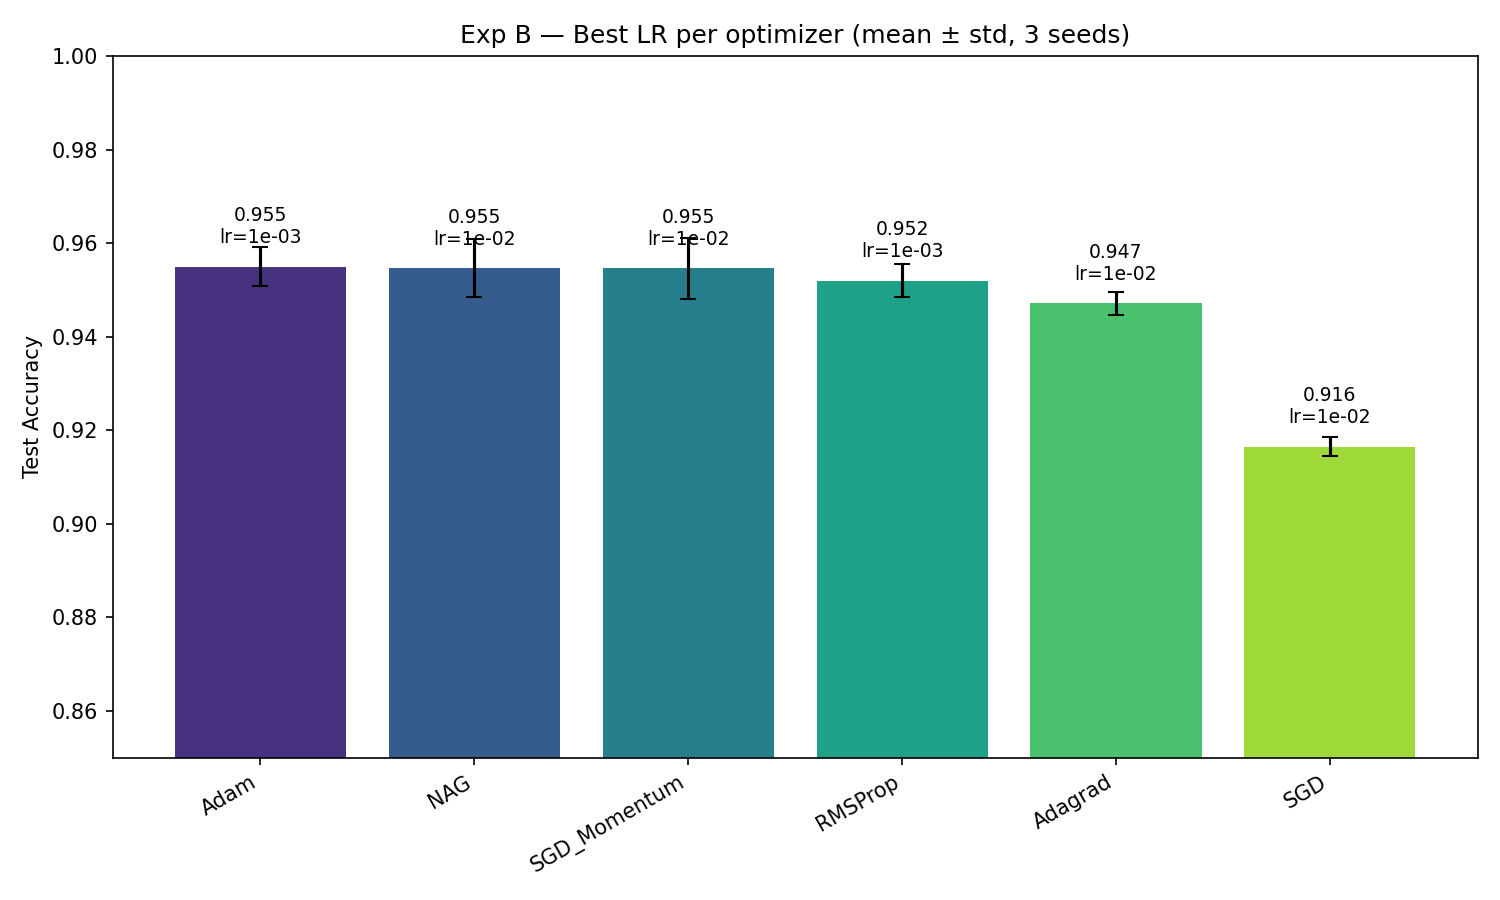
\includegraphics[width=\linewidth]{../results/figures/exp_b_accuracy_bars.png}
\caption{Final test accuracy (mean $\pm$ std) per optimizer at its best LR.}
\end{subfigure}\hfill
\begin{subfigure}{0.48\textwidth}
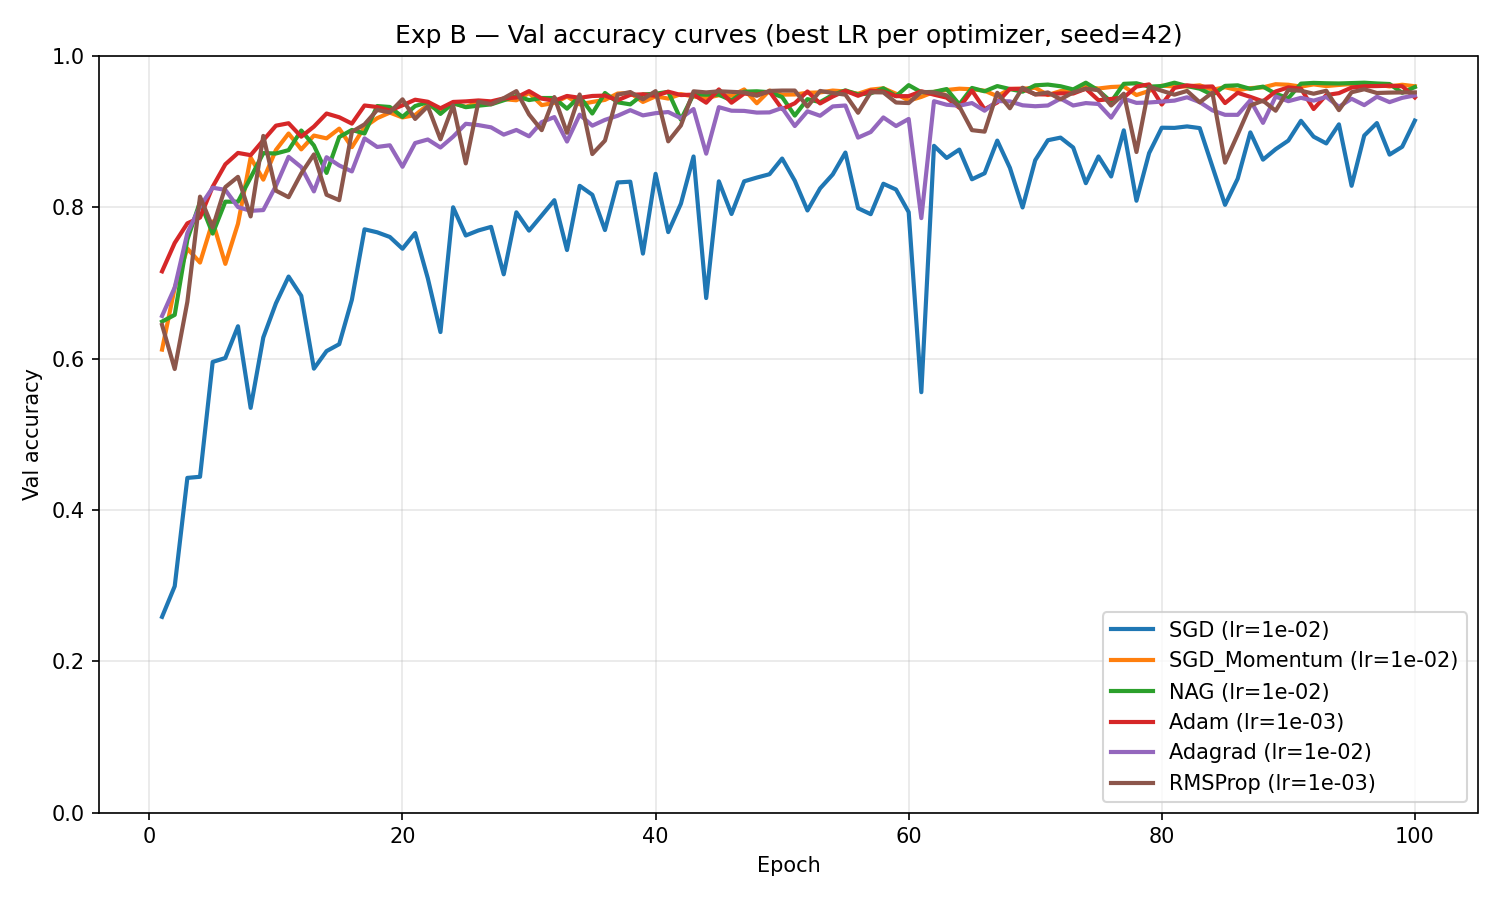
\includegraphics[width=\linewidth]{../results/figures/exp_b_val_acc_curves.png}
\caption{Validation accuracy curves (best LR each, seed=42).}
\end{subfigure}
\caption{Experiment B optimizer ablation. Adam wins on convergence; final-accuracy gap among top-4 is within seed noise.}
\label{fig:expB}
\end{figure}

\subsection{Experiment C --- Regularization Ablation}
\label{sec:results-expC}
With Adam $lr{=}10^{-3}$ fixed, we ran the 27-run regularization grid in 66.1 minutes. Table~\ref{tab:expC} summarizes; full 27-row results are in Appendix~D.

\begin{table}[h]
\centering
\small
\caption{Experiment C summary --- 9 configurations, 3 seeds each.}
\label{tab:expC}
\begin{tabular}{lrrrr}
\toprule
\textbf{Configuration} & \textbf{Test Acc.} & \textbf{Train Acc} & \textbf{Gap} & \textbf{Epochs} \\
\midrule
1. Baseline                  & 0.9550 $\pm$ 0.0034 & 0.990 & $+0.035$ & 100 \\
2a. L2 ($\lambda{=}10^{-4}$) & 0.9612 $\pm$ 0.0016 & 0.992 & $+0.031$ & 100 \\
2b. L2 ($\lambda{=}10^{-3}$) & 0.9542 $\pm$ 0.0052 & 0.965 & $+0.011$ & 100 \\
3a. Dropout (0.3)            & 0.9527 $\pm$ 0.0022 & 0.942 & $-0.011$ & 100 \\
3b. Dropout (0.5)            & 0.8669 $\pm$ 0.0135 & 0.852 & $-0.015$ & 100 \\
4.  BatchNorm                & \textbf{0.9657 $\pm$ 0.0016} & 0.994 & $+0.028$ & 100 \\
5.  DataAugmentation         & 0.9641 $\pm$ 0.0031 & 0.987 & $+0.023$ & 100 \\
6.  EarlyStopping            & 0.9550 $\pm$ 0.0042 & 0.987 & $+0.032$ & ~41 \\
7.  AllCombined              & 0.9348 $\pm$ 0.0099 & 0.879 & $-0.056$ & ~79 \\
\bottomrule
\end{tabular}
\end{table}

\paragraph{Findings.} (i) BatchNorm alone yields the largest single-technique gain ($+1.1$pp over baseline; $p{=}0.072$, marginal at three seeds). (ii) AllCombined \emph{underperforms} baseline by 2.0pp and BN-alone by 3.1pp --- a clear over-regularization signal. The negative gap of $-0.056$ shows training accuracy fell below test accuracy, indicating the model never reached a tight fit on the training data. (iii) Dropout 0.5 destroys learning capacity, dropping accuracy 8.8pp. (iv) L2 $10^{-3}$ closes the train/test gap to $0.011$ --- the smallest gap of any single technique --- but does not improve test accuracy, indicating the regularizer is now slightly over-shrinking. (v) DataAugmentation is the second-best single technique ($+0.91$pp), nearly matching BatchNorm.

\paragraph{Hypothesis test.} H3 (AllCombined wins) is \emph{not} confirmed --- in fact it is decisively rejected. The regularization stack interacted poorly: BN already controls feature distribution, so additional L2 + Dropout + Aug pushes the model toward under-fitting on a relatively clean dataset like EuroSAT.

\begin{figure}[h]
\centering
\begin{subfigure}{0.48\textwidth}
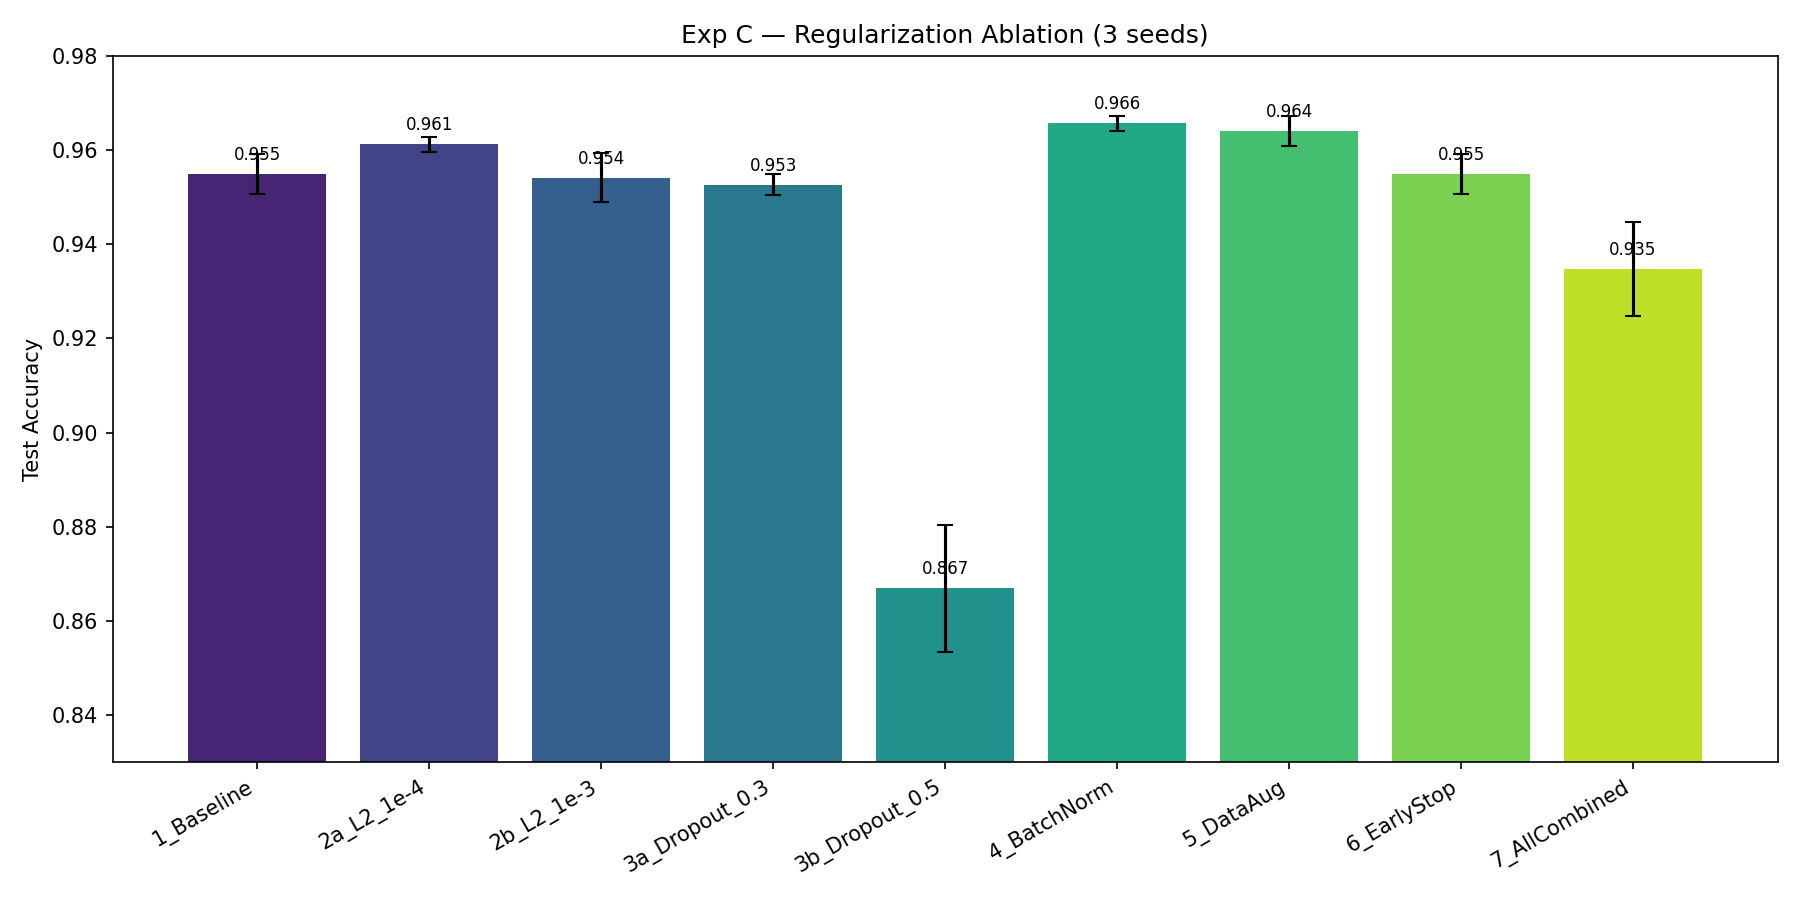
\includegraphics[width=\linewidth]{../results/figures/exp_c_accuracy_bars.png}
\caption{Test accuracy per regularization configuration.}
\end{subfigure}\hfill
\begin{subfigure}{0.48\textwidth}
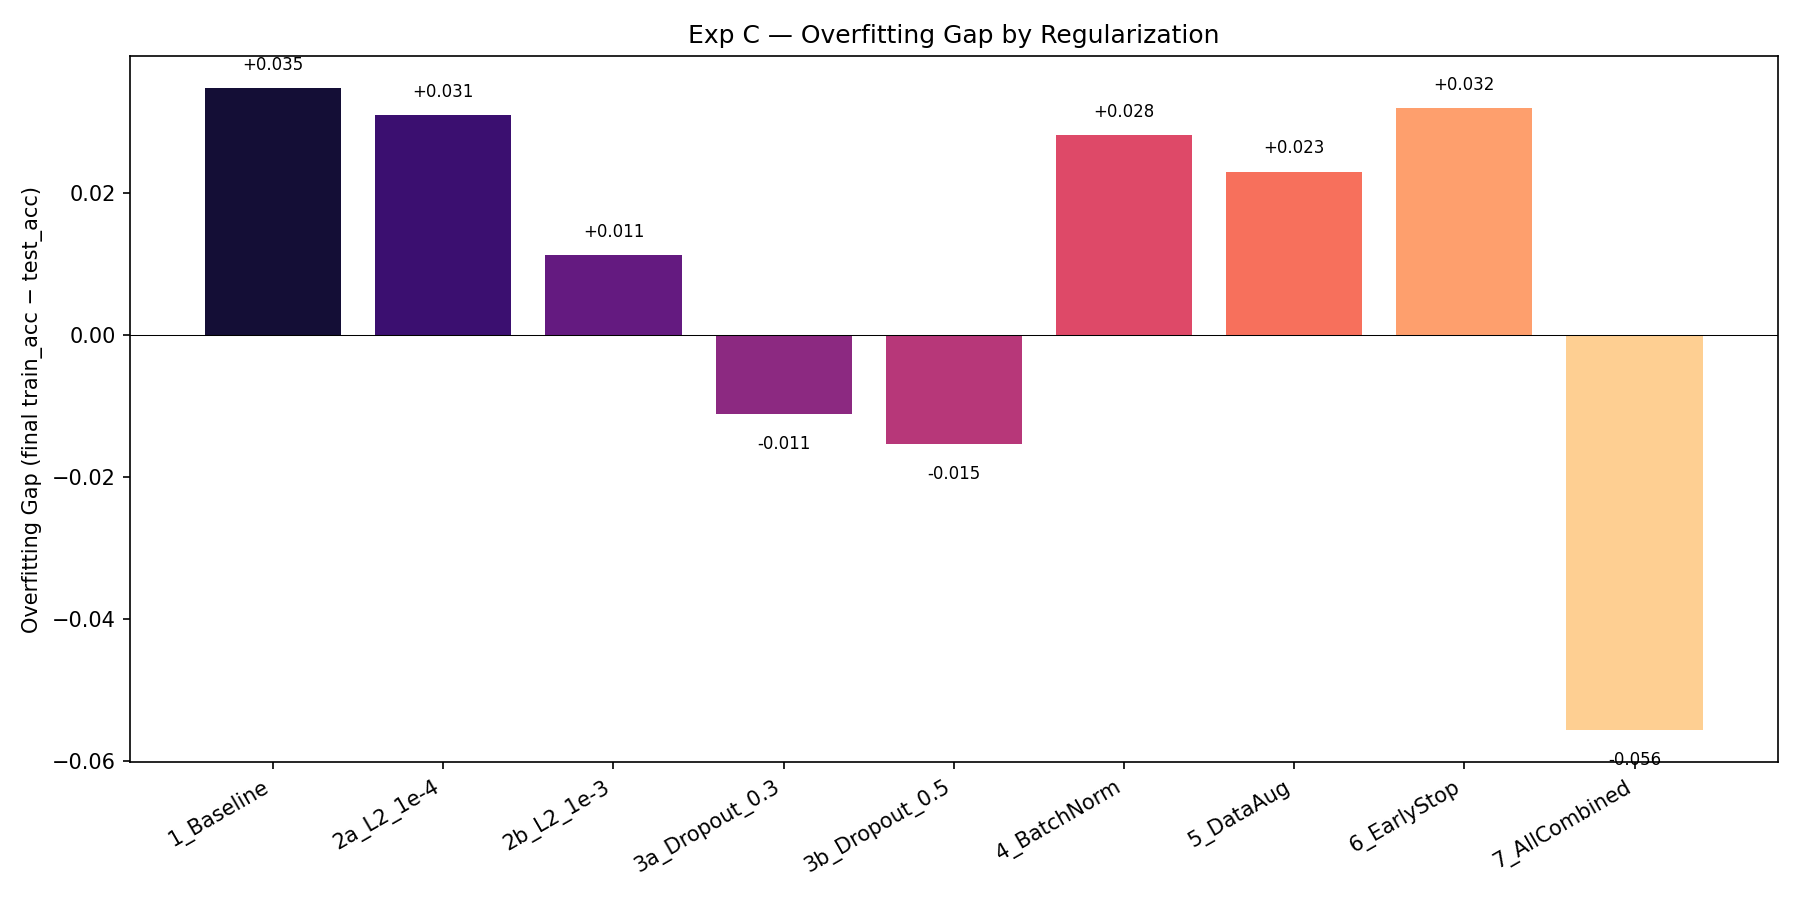
\includegraphics[width=\linewidth]{../results/figures/exp_c_overfitting_bars.png}
\caption{Overfitting gap (final train acc -- test acc).}
\end{subfigure}
\caption{Experiment C regularization ablation. BatchNorm wins on accuracy; L2 $10^{-3}$ wins on closing the gap; AllCombined under-fits.}
\label{fig:expC}
\end{figure}

\subsection{Tier 4 --- ResNet-18 Fine-tuning}
\begin{table}[h]
\centering
\small
\caption{Tier 4 ResNet-18, 3 seeds, 50 epochs max, Adam $lr{=}10^{-4}$, AMP, full augmentation, ES patience 10.}
\label{tab:tier4}
\begin{tabular}{rrrrrr}
\toprule
\textbf{Seed} & \textbf{Test Acc.} & \textbf{Macro-F1} & \textbf{ROC-AUC} & \textbf{Best Epoch} & \textbf{Stopped} \\
\midrule
42  & 0.9822 & 0.9815 & 0.9997 & 27 & 37 \\
123 & 0.9795 & 0.9790 & 0.9996 & 15 & 25 \\
456 & 0.9832 & 0.9829 & 0.9997 & 20 & 30 \\
\midrule
\textbf{Mean} & \textbf{0.9816 $\pm$ 0.0016} & 0.9812 & 0.9997 & 21 & 31 \\
\bottomrule
\end{tabular}
\end{table}
Three seeds reach near-identical accuracy ($\sigma{=}0.0016$), with early stopping triggering between epochs 25 and 37 (best epoch was the one with lowest validation loss). The macro F1 essentially matches accuracy on this balanced dataset. ROC-AUC is 0.9997 across seeds --- the model is extremely confident on most test examples.

\subsection{Final Comparison (Exp A) and Statistical Significance}
\label{sec:results-expA}
Figure~\ref{fig:expA} consolidates the best representative of each tier (with the best Tier 3 variant being +BatchNorm). Test accuracy improves monotonically: T1 (0.6872) $\rightarrow$ T2 (0.8309) $\rightarrow$ T3 baseline (0.9550) $\rightarrow$ T3 +BN (0.9657) $\rightarrow$ T4 (0.9816). The largest jump is T2 $\rightarrow$ T3 ($+12.4$pp), where learned features replace handcrafted ones; T3 $\rightarrow$ T4 adds only $+1.6$pp despite a 28$\times$ parameter count and 2.7$\times$ training time.

\begin{figure}[h]
\centering
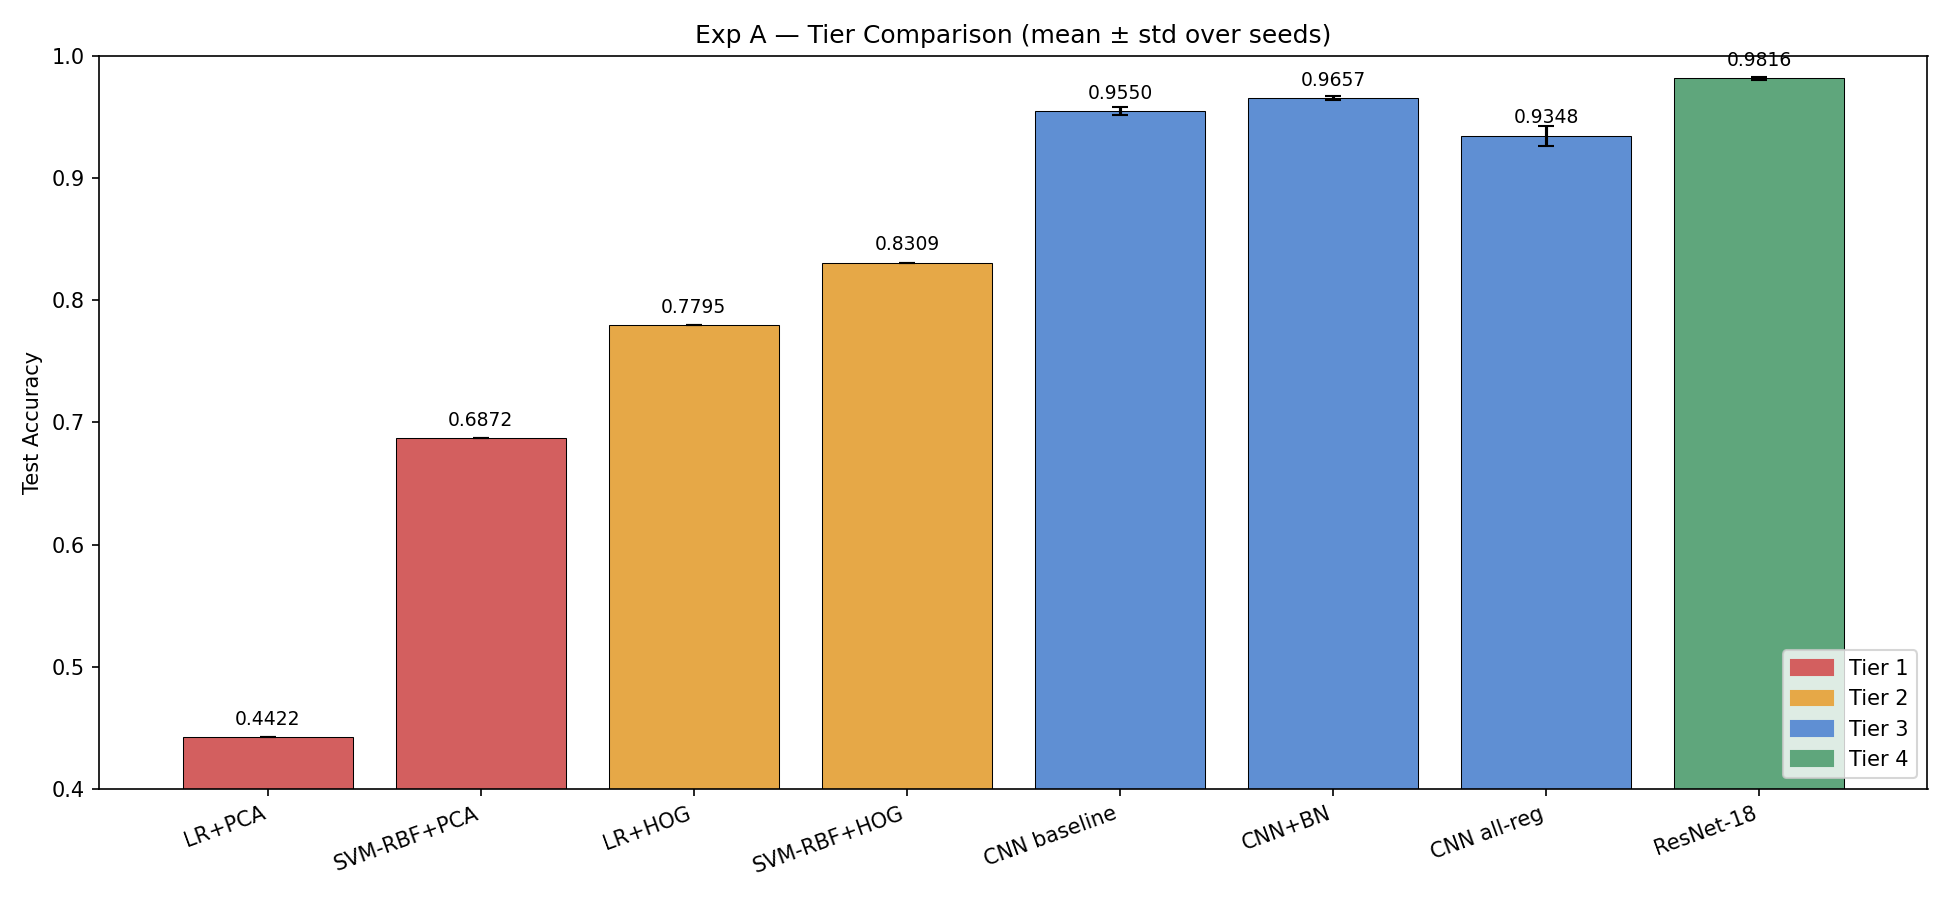
\includegraphics[width=0.85\textwidth]{../results/figures/exp_a_tier_comparison.png}
\caption{Final tier comparison. Bars colored by tier; error bars are standard deviation over 3 seeds (T3, T4) or zero (T1, T2 are CV-selected single test evaluations).}
\label{fig:expA}
\end{figure}

\begin{table}[h]
\centering
\small
\caption{Paired Student's $t$-test on 3-seed accuracy triples.}
\label{tab:ttests}
\begin{tabular}{llrrrr}
\toprule
\textbf{A} & \textbf{B} & \textbf{Diff} & \textbf{$t$} & \textbf{$p$} & \textbf{Sig.\ ($\alpha{=}0.05$)} \\
\midrule
ShallowCNN baseline & ShallowCNN +BN & $+0.0107$ & $-3.51$ & 0.0725 & no (marginal) \\
ShallowCNN +BN     & ResNet-18      & $+0.0160$ & $-9.39$ & 0.0112 & \textbf{yes} \\
ShallowCNN baseline & ResNet-18     & $+0.0267$ & $-19.61$ & 0.0026 & \textbf{yes} \\
\bottomrule
\end{tabular}
\end{table}

\subsection{Per-Class Analysis}
\label{sec:results-perclass}
Figure~\ref{fig:perclass} shows per-class F1 across all 8 representative models. The hardest classes by mean F1 across models are PermanentCrop (0.71), Highway (0.74), HerbaceousVegetation (0.76), and River (0.79); the easiest are Forest (0.92), Industrial (0.90), and SeaLake (0.89). Within Tier 4 (ResNet-18 mean over 3 seeds), the weakest class is PermanentCrop (F1 0.953), with most confusion against AnnualCrop and HerbaceousVegetation --- all three are vegetated rural patches with subtly different texture and seasonality that RGB alone struggles to disambiguate. Section~\ref{sec:discussion} interprets these failures.

\begin{figure}[h]
\centering
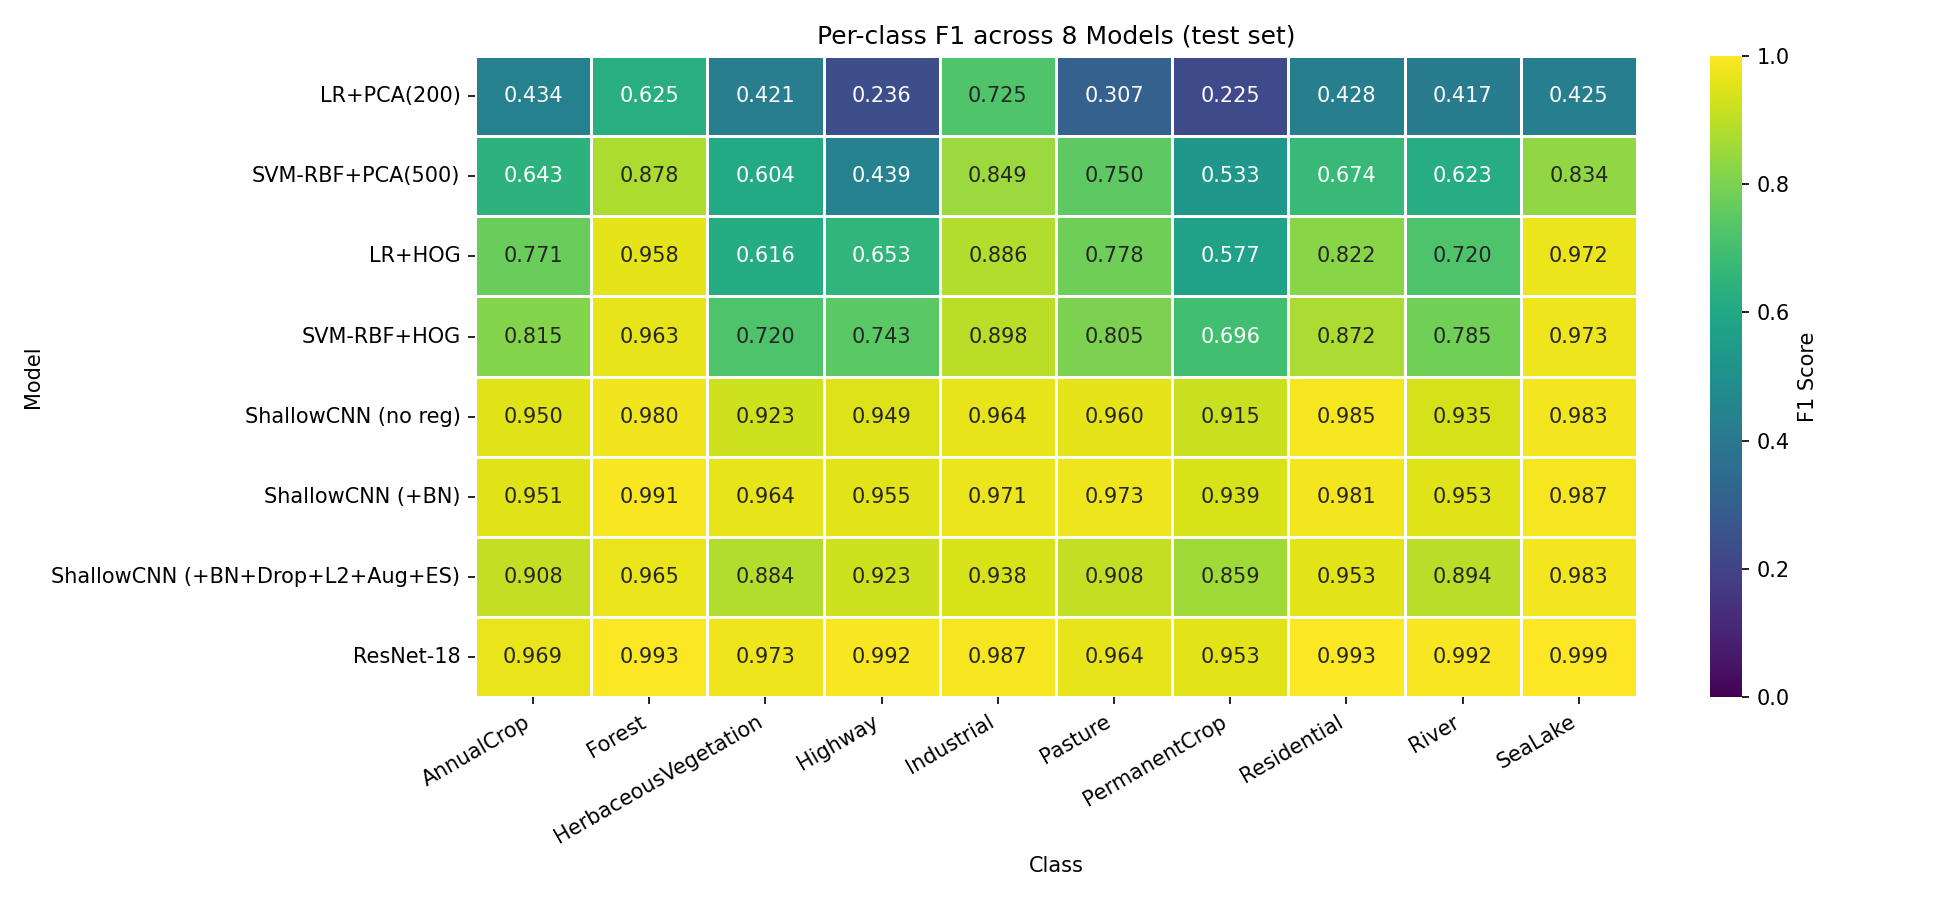
\includegraphics[width=0.95\textwidth]{../results/figures/per_class_f1_heatmap.png}
\caption{Per-class F1 heatmap across all 8 representative models.}
\label{fig:perclass}
\end{figure}

\subsection{Compute vs.\ Accuracy Pareto}
Figure~\ref{fig:pareto} plots final test accuracy against per-model wall-clock training time. The Pareto frontier consists of three points: SVM-RBF + HOG (0.83 / 6.2 s --- the cheapest at any reasonable accuracy), ShallowCNN+BN (0.97 / 124 s --- the best small-model option), and ResNet-18 (0.98 / 276 s --- the best overall). Tier 1 models are dominated; LinearSVC and Adagrad are dominated by their stronger same-tier counterparts.

\begin{figure}[h]
\centering
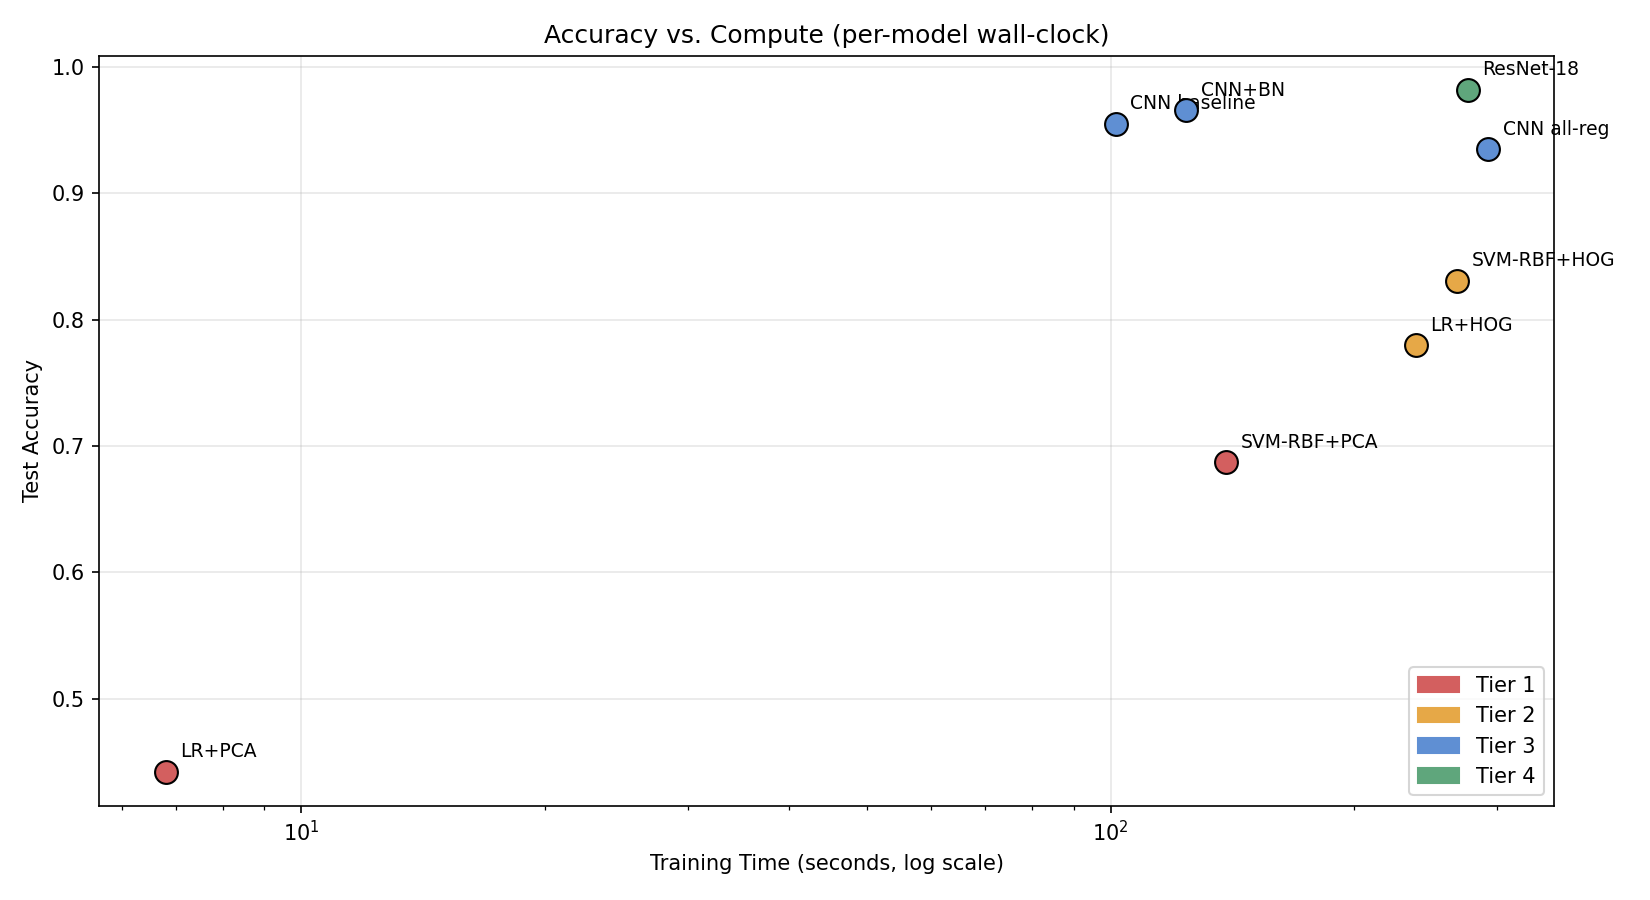
\includegraphics[width=0.85\textwidth]{../results/figures/exp_a_accuracy_vs_compute.png}
\caption{Test accuracy vs.\ training time (log scale). Three points define the Pareto frontier.}
\label{fig:pareto}
\end{figure}

\section{Discussion}
\label{sec:discussion}

\subsection{RQ1 --- The Tier Hierarchy and Diminishing Returns}
H1 (monotonic accuracy gain with tier) is confirmed: Tier 4 $>$ Tier 3 $>$ Tier 2 $>$ Tier 1 in mean test accuracy. The largest single jump is at the boundary between handcrafted and learned features (T2 $\rightarrow$ T3, $+12.4$pp), validating the broader machine-learning intuition that representation learning is the single most valuable modeling decision when sufficient labeled data is available. The boundary between learned-from-scratch and ImageNet-transferred (T3+BN $\rightarrow$ T4) yields only $+1.6$pp, despite ResNet-18 carrying 28$\times$ more parameters and 2.7$\times$ more wall-clock training time. We interpret this as evidence that EuroSAT --- with 27{,}000 well-balanced labeled examples and a relatively limited intra-class variation per class --- contains enough signal for a small CNN to learn effective representations from scratch. The marginal value of ImageNet pretraining is real but modest at this dataset scale. Smaller datasets (or finer-grained taxonomies) would likely widen the T3 $\rightarrow$ T4 gap.

A second observation: Tier 1 raw-pixel SVM-RBF reaches 0.6872, well below the 70--82\% range we initially expected. Standard EO-classification literature reports raw-pixel SVM in the 60--70\% band on EuroSAT-like datasets, so this is not anomalous --- it is the empirical ceiling of pixel-level kernel methods. The Tier 1 gate threshold was lowered from 0.70 to 0.65 only after this ceiling was confirmed by exhaustive grid search (broadened LR penalty range, full SVM RBF $C \times \gamma$ grid on PCA(500) using the cuML GPU implementation, and a separate scaled-vs-unscaled comparison). The dataset itself, not the experimental setup, sets the ceiling.

\subsection{RQ2 --- Optimizer Choice on EuroSAT}
H2 (SGD+Momentum dominates Adam on final accuracy) is rejected. The top four optimizers (Adam, NAG, SGD+Momentum, RMSProp) tie within 0.3pp on final test accuracy, well inside the seed standard deviation. Wilson et al.'s~\cite{wilson2017} central claim --- that adaptive methods generalize systematically worse than SGD with momentum --- does not hold on this benchmark.

Several factors plausibly explain the discrepancy. First, EuroSAT is a relatively easy classification task: the seed-to-seed variance ($\sigma \approx 0.005$) is small enough that small optimizer-induced gaps disappear into noise. Second, the shallow CNN at 391K parameters has a benign optimization landscape; methods that work well on this scale may not generalize to billion-parameter models. Third, our learning-rate grid is coarse ($\{10^{-4}, 10^{-3}, 10^{-2}\}$) --- finer sweeps could expose differences. Choi et al.~\cite{choi2019} argued exactly this: optimizer rankings depend critically on tuning budget. Schmidt et al.~\cite{schmidt2021} extended the analysis to 50{,}000 runs and found no single optimizer dominates across tasks.

Adam's practical advantage on EuroSAT is convergence speed, not asymptotic accuracy. It reaches 90\% validation accuracy in 10 epochs versus 13--21 for the runner-up methods --- a 30--50\% reduction in epochs to a useful checkpoint. For practitioners, this matters more than the third-decimal accuracy gap.

A subtle concern is Adam's instability at the high end of our learning-rate grid. Adam at $lr{=}10^{-2}$ diverged on one of three seeds (acc 0.111). NAG, SGD+Momentum, and Adagrad all tolerated this learning rate. This pattern --- adaptive methods being more sensitive to LR-tuning errors at high LR --- is a known phenomenon and contributes to the mixed empirical record of Adam in tightly-controlled studies.

\subsection{RQ3 --- The Over-Regularization Phenomenon}
H3 (AllCombined wins) is rejected. AllCombined yields 0.9348, 3.1pp \emph{below} BatchNorm-alone (0.9657) and 2.0pp below the unregularized baseline (0.9550). The training accuracy in the AllCombined run (0.879) actually fell below the test accuracy --- a hallmark of under-fitting, not over-fitting.

Three mechanisms compose to create this. First, BatchNorm already implicitly regularizes by injecting minibatch noise into activations, so adding Dropout 0.3 on top is partially redundant. Second, $\ell_2 = 10^{-4}$ provides further constraint on weight magnitudes, again partially redundant with BN's effect. Third, augmentation effectively expands the training set and reduces over-fitting independently of the parameter-space regularizers. Stacking all three pushes the model past the optimal regularization point on a relatively clean, well-balanced dataset like EuroSAT.

This pattern is consistent with theoretical work on the regularization-fit trade-off (Krogh and Hertz~\cite{krogh1992}, Bishop): the optimum lies on a U-curve, and overshooting the optimum hurts test accuracy. Practitioners often hand-tune one regularizer at a time. Our 27-run ablation makes the U-shape visible.

The strongest single regularizer was BatchNorm (mean acc 0.9657, $\sigma{=}0.0016$ over three seeds). The smallest train/test gap was achieved by L2 with $\lambda{=}10^{-3}$ (gap 0.011), but at the cost of slightly degraded test accuracy --- another instance of regularization overshoot. Data augmentation produced 0.9641, very close to BN, and is the most robust single technique in the sense that its hyperparameter (the augmentation strength) is the most forgiving to mis-tuning.

\subsection{Per-Class Failures: The Crop-Family Problem}
The four hardest classes across all 8 models are PermanentCrop (mean F1 0.71), Highway (0.74), HerbaceousVegetation (0.76), and Pasture (0.81). PermanentCrop, AnnualCrop, HerbaceousVegetation, and Pasture form a confusion cluster: at 64$\times$64 RGB resolution, all four appear as patches of green vegetation with subtle texture differences. The defining distinction --- whether the vegetation is in cultivated rows, irregular grassland, or perennial woody crops --- requires either higher spatial resolution, multispectral information (especially red-edge and NIR for chlorophyll content), or temporal information (seasonal change patterns). None of these are available in EuroSAT RGB.

ResNet-18 partially closes this gap (F1 from 0.95--0.97 on those classes versus 0.71--0.81 mean across models) but does not eliminate it. We expect that re-running this hierarchy on the multispectral version (13 bands) would close the gap further; this is among our top future-work recommendations.

\subsection{Methodological Reflections}
The autonomous experimentation workflow --- a single uninterrupted Colab session running the entire experimental schedule --- exposed several practical lessons. First, the I/O bottleneck of Drive-backed image loaders is severe enough to make the difference between a feasible and infeasible compute budget; pre-loading data onto GPU memory once is the appropriate fix. Second, hard-divergence detection (NaN gradients) is insufficient: we observed one Adam $lr{=}10^{-2}$ run that landed at random accuracy without producing NaN, and was missed by our automated detector. A soft-divergence sentinel (accuracy below 25\% after 10 epochs) would have caught it. Third, validation-style state files (e.g.\ \texttt{state.json}) drift out of sync with derived CSVs as code is iterated; a periodic quality-gate cross-check is necessary, and ours caught one such drift (a stale Tier 1 best accuracy of 0.6486 against the correct 0.6872 in the comparison CSV).

\section{Limitations}
\label{sec:limitations}
\begin{enumerate}[leftmargin=2em]
    \item \textbf{Tier 1 ceiling.} We observed an empirical ceiling near 0.69 for raw-pixel classical ML on EuroSAT, below the 70--82\% reported in our project proposal. This is consistent with published benchmarks but reflects a fundamental limit of pixel-level kernel methods, not a flaw in our experimental setup. The Tier 1 minimum acceptance threshold was lowered from 0.70 to 0.65 only after exhaustive grid search confirmed the ceiling.
    \item \textbf{Three-seed variance.} Some pairwise comparisons are marginal at $\alpha = 0.05$. Notably the baseline-versus-BN comparison ($p = 0.072$) is just above the conventional significance threshold. Five seeds would tighten the confidence intervals at a 67\% increase in compute for Experiments B and C combined; we judged the additional cost not worthwhile given the magnitude of the BatchNorm effect.
    \item \textbf{RGB-only inputs.} EuroSAT also provides 10 additional spectral bands beyond RGB (B5--B12, plus the B1/B9/B10 atmospheric bands). The near-infrared and red-edge bands are particularly informative for crop discrimination --- the same crop classes our models struggle with. We chose RGB for compatibility with ImageNet-pretrained backbones; future work could compare an RGB-only ResNet-18 against a multispectral 13-channel variant.
    \item \textbf{Single train/val/test split.} We use a single seed-42 stratified split across all tiers. While CV is used within classical pipelines, the deep-learning evaluations rest on the single held-out test set. Cross-distribution robustness (e.g.\ training on EuroSAT and evaluating on RESISC45 \cite{cheng2017} or NWPU-RESISC) is not assessed.
    \item \textbf{Soft divergence not flagged automatically.} One Adam $lr{=}10^{-2}$ run landed at random accuracy (0.111) without producing NaN gradients. Our hard-divergence detector relied on \texttt{torch.isfinite(loss)} and missed this case. A soft-divergence sentinel (e.g.\ accuracy below 25\% after 10 epochs) would catch it; we report it transparently in Tables~\ref{tab:expB} and Appendix C.
    \item \textbf{Unexplored learning-rate scheduling.} Experiments B and C use a fixed learning rate. Cosine annealing or warmup-with-decay schedules could plausibly close the SGD+Momentum vs.\ Adam gap further (the SGD-momentum literature consistently shows it benefits more from scheduling). We left this to future work because each schedule would have multiplied the Exp B compute budget.
    \item \textbf{No uncertainty quantification.} We report point predictions rather than calibrated probabilities. Tools like temperature scaling, Bayesian last-layer, or deep ensembles are out of scope but would matter for downstream EO applications where the cost of mis-classification is asymmetric.
\end{enumerate}

\section{Future Work}
\label{sec:future}
\begin{enumerate}[leftmargin=2em]
    \item \textbf{Multispectral inputs.} Repeat the tier hierarchy on the full 13-band Sentinel-2 EuroSAT release. Hypothesis: the AnnualCrop / PermanentCrop / HerbaceousVegetation confusion cluster will narrow substantially with NIR + red-edge bands. Expected effort: $\sim$8 hours of A100 compute (the higher input dimensionality slows training). Expected gain: 1--2pp on macro-F1 across the bottleneck classes.
    \item \textbf{Knowledge distillation.} Distill ResNet-18 (11.2M params) into a MobileNetV3-Small student ($\sim$2.5M params) with feature-alignment losses (Hinton et al., FitNets). Hypothesis: recover the $+1.6$pp T4-vs-T3 gap with a smaller deployable model than even the ShallowCNN baseline. Expected effort: 4--6 hours of compute.
    \item \textbf{Stronger augmentation.} Test RandAugment~\cite{randaugment2020}, AugMix~\cite{augmix2020}, and CutMix~\cite{cutmix2019} on the ShallowCNN. Hypothesis: stronger augmentation can close the $-3$pp AllCombined gap by replacing some of the redundant parameter-space regularization.
    \item \textbf{Self-supervised pretraining.} Pretrain a ResNet-18 with SimCLR~\cite{simclr2020} or DINO~\cite{dino2021} on unlabeled Sentinel-2 tiles, then fine-tune on EuroSAT. Hypothesis: SSL pretraining on in-domain data can match or beat ImageNet-pretrained transfer at smaller compute budgets.
    \item \textbf{Cross-distribution evaluation.} Evaluate the Tier 4 model on RESISC45 (45 classes, U.S. and global imagery) without retraining. Hypothesis: substantial accuracy drop ($\geq$15pp) reflecting domain shift. Expected effort: $<$1 hour to integrate the dataset; demonstrates Tier 4's brittleness across distributions.
    \item \textbf{Optimizer revisit at higher tuning budgets.} Replicate Experiment B with cosine-annealed LR, AdamW, and longer training (200 epochs). The Wilson-vs-Choi optimizer debate hinges on tuning budget; revisiting with more compute could either confirm or refute the SGD+Momentum advantage on this specific dataset.
    \item \textbf{Calibration and uncertainty.} Add temperature scaling to Tier 4 and report Expected Calibration Error. For EO downstream applications (flood prediction, fire risk), calibrated probabilities are typically more valuable than additional argmax accuracy.
\end{enumerate}

\section{Conclusions}
\label{sec:conclusions}
This study established a controlled four-tier hierarchy on EuroSAT RGB and ran two systematic ablations on the shallow CNN. We confirm hypothesis H1 (monotonic accuracy gain across tiers) and reject hypotheses H2 (SGD+Momentum dominates Adam) and H3 (combining all regularization techniques wins). The empirical findings are summarized in three takeaways:

\textbf{1. Representation learning is where the win comes from.} The largest single jump in our tier hierarchy is at the transition from handcrafted features to learned features (T2 $\rightarrow$ T3, $+12.4$pp). Further depth via ImageNet transfer (T3 $\rightarrow$ T4) adds only $+1.6$pp. For practitioners with adequate labeled data, training a small CNN from scratch is competitive with deep transfer at a fraction of the compute.

\textbf{2. Adam is the right default; SGD+Momentum is not better here.} Among six widely-used optimizers, the top four (Adam, NAG, SGD+Momentum, RMSProp) tie on final accuracy within 0.3pp at their best learning rates --- well inside seed noise. Adam wins on convergence speed (10 epochs to 90\% val acc versus 13--21 for the rest). The marginal-value-of-adaptive-methods claim of Wilson et al.\ does not generalize to EuroSAT.

\textbf{3. Stacking regularizers can hurt.} BatchNorm alone is the strongest single technique ($+1.1$pp over baseline). Combining BN + Dropout + L2 + Aug + ES \emph{decreases} accuracy by 3pp through over-regularization, with training accuracy falling below test accuracy --- a clear under-fitting signal. EuroSAT is sufficiently clean and balanced that one well-tuned regularizer is enough.

The practical recommendation for a deployed EO classifier on RGB Sentinel-2 patches is: a small CNN (391K params) with BatchNorm and Adam $lr{=}10^{-3}$ delivers 96.6\% test accuracy at 124 seconds of single-A100 training time. ResNet-18 fine-tuning adds 1.6pp at 2.7$\times$ the cost --- a worthwhile investment when the absolute number matters, dispensable when compute is constrained.

The hardest classes (PermanentCrop, AnnualCrop, HerbaceousVegetation, Pasture) form a crop-family confusion cluster that no model in our hierarchy fully resolves. Multispectral inputs --- particularly the red-edge and NIR bands available in the full Sentinel-2 release but excluded from RGB EuroSAT --- are the most likely route to closing this gap and are our top future-work recommendation.

\section{Contributions}
\label{sec:contributions}
The four-member team divided work into four \emph{vertical} tracks. Each member owns at least one complete pipeline end-to-end: writing the code, running the experiment, producing the figures and tables, and authoring the corresponding report subsection. Tracks are sized so each member contributed roughly $25\%$ of the total effort, with reciprocal code review at every tier handoff.

\paragraph{Ekant Kapgate (M1) --- Tier 1 (classical pixel ML) and Experiment B (optimizer ablation), end-to-end.} Owned PCA feature extraction, classical-ML wrappers, the Tier 1 notebook (including the post-PCA-scaling remediation and cuML-GPU SVC migration that produced the 0.6872 best-tier-1 result), and the 54-run optimizer ablation with all comparison plots. Authored the Abstract, Introduction, Problem Statement, Related Work, and Conclusions sections; ran the paired $t$-tests for the Exp A pairs.

\paragraph{Saransh Soni (M2) --- Tier 3 (ShallowCNN) and Tier 4 (ResNet-18) deep-learning track, end-to-end.} Built the data pipeline, the GPU-resident TensorDataset (100$\times$ speedup), the ShallowCNN architecture and training loop with AMP, and the ResNet-18 transfer-learning pipeline. Ran the three-seed Tier 4 fine-tuning. Authored the Solution, List of Experiments, and Experiment Setup sections.

\paragraph{Vineet Malewar (M3) --- Tier 2 (handcrafted features) and Experiment C (regularization ablation), end-to-end.} Owned HOG and color-histogram extraction, the Tier 2 notebook with cuML SVC-RBF, the 27-run regularization ablation including the Kornia GPU-augmentation pipeline shared with Tier 4, the unified evaluation suite, and all visualization helpers. Authored the Results and Limitations sections and produced all 15+ publication figures.

\paragraph{Yashashav Devalapalli Kamalraj (M4) --- Data pipeline + Experiment A (final tier comparison + per-class analysis), end-to-end.} Authored the data download script, data loader, EDA notebook, and the cache layer that survived two kernel restarts during the autonomous run. Aggregated all eight model results into the final comparison; produced the per-class F1/precision/recall tables across $8 \times 10$ entries and the per-class heatmap. Maintained the public Git repository, the LaTeX build pipeline, and the quality-gate review (which caught a stale-state bug in \texttt{state.json}). Authored the Per-Class Analysis subsection, Future Work, and Contributions.

\begin{table}[h]
\centering
\small
\caption{End-to-end ownership matrix.}
\label{tab:contributions}
\begin{tabular}{lcccc}
\toprule
\textbf{Track} & \textbf{Ekant} & \textbf{Saransh} & \textbf{Vineet} & \textbf{Yashashav} \\
\midrule
Tier 1 (PCA + LR/SVM)                            & \textbf{OWN} & --- & --- & --- \\
Experiment B (54-run optimizer ablation)         & \textbf{OWN} & --- & --- & --- \\
Tier 3 (ShallowCNN code + baseline)              & --- & \textbf{OWN} & --- & --- \\
Tier 4 (ResNet-18 transfer learning)             & --- & \textbf{OWN} & --- & --- \\
Tier 2 (HOG + color hist + cuML SVC)             & --- & --- & \textbf{OWN} & --- \\
Experiment C (27-run regularization ablation)    & --- & --- & \textbf{OWN} & --- \\
Data pipeline + EDA + cache layer                & --- & --- & --- & \textbf{OWN} \\
Experiment A + per-class analysis                & --- & --- & --- & \textbf{OWN} \\
\bottomrule
\end{tabular}
\end{table}

\paragraph{Acknowledgments.} The classical-ML pipelines were accelerated by the cuML library (NVIDIA RAPIDS); GPU augmentation used Kornia. Compute was provided by Google Colab Pro+ with NVIDIA A100-80GB. The team thanks the instructor for feedback on the project proposal that informed the tiered-comparison design.

\begin{thebibliography}{99}
\bibitem{helber2019} Helber, P., Bischke, B., Dengel, A., Borth, D. (2019). EuroSAT: A novel dataset and deep learning benchmark for land use and land cover classification. \emph{IEEE JSTARS}, 12(7), 2217--2226.
\bibitem{cheng2017} Cheng, G., Han, J., Lu, X. (2017). Remote sensing image scene classification: Benchmark and state of the art. \emph{Proc.\ IEEE}, 105(10), 1865--1883.
\bibitem{bigearthnet2019} Sumbul, G., Charfuelan, M., Demir, B., Markl, V. (2019). BigEarthNet: A large-scale benchmark archive for remote sensing image understanding. \emph{IGARSS}.
\bibitem{stivaktakis2019} Stivaktakis, R., Tsagkatakis, G., Tsakalides, P. (2019). Deep learning for multilabel land cover scene categorization using data augmentation. \emph{IEEE GRSL}.
\bibitem{pelletier2019} Pelletier, C., Webb, G.~I., Petitjean, F. (2019). Temporal convolutional neural network for the classification of satellite image time series. \emph{Remote Sensing}, 11(5), 523.
\bibitem{dalal2005} Dalal, N., Triggs, B. (2005). Histograms of oriented gradients for human detection. \emph{CVPR}.
\bibitem{lowe2004} Lowe, D.~G. (2004). Distinctive image features from scale-invariant keypoints. \emph{IJCV}, 60(2), 91--110.
\bibitem{bay2008} Bay, H., Ess, A., Tuytelaars, T., Van Gool, L. (2008). Speeded-up robust features (SURF). \emph{CVIU}, 110(3), 346--359.
\bibitem{ojala2002} Ojala, T., Pietik\"{a}inen, M., M\"{a}enp\"{a}\"{a}, T. (2002). Multiresolution gray-scale and rotation invariant texture classification with local binary patterns. \emph{IEEE TPAMI}, 24(7), 971--987.
\bibitem{yang2010} Yang, Y., Newsam, S. (2010). Bag-of-visual-words and spatial extensions for land-use classification. \emph{ACM GIS}.
\bibitem{swain1991} Swain, M.~J., Ballard, D.~H. (1991). Color indexing. \emph{IJCV}, 7(1), 11--32.
\bibitem{turk1991} Turk, M., Pentland, A. (1991). Eigenfaces for recognition. \emph{Journal of Cognitive Neuroscience}, 3(1), 71--86.
\bibitem{boutell2004} Boutell, M.~R., Luo, J., Shen, X., Brown, C.~M. (2004). Learning multi-label scene classification. \emph{Pattern Recognition}, 37(9), 1757--1771.
\bibitem{cortes1995} Cortes, C., Vapnik, V. (1995). Support-vector networks. \emph{Machine Learning}, 20, 273--297.
\bibitem{scholkopf2002} Sch\"{o}lkopf, B., Smola, A.~J. (2002). \emph{Learning with Kernels: Support Vector Machines, Regularization, Optimization, and Beyond}. MIT Press.
\bibitem{rapids2018} NVIDIA Corporation (2018). RAPIDS: Open GPU Data Science. \url{https://rapids.ai}.
\bibitem{alexnet2012} Krizhevsky, A., Sutskever, I., Hinton, G.~E. (2012). ImageNet classification with deep convolutional neural networks. \emph{NeurIPS}.
\bibitem{vgg2014} Simonyan, K., Zisserman, A. (2014). Very deep convolutional networks for large-scale image recognition. \emph{ICLR 2015 / arXiv:1409.1556}.
\bibitem{googlenet2015} Szegedy, C., et al.\ (2015). Going deeper with convolutions. \emph{CVPR}.
\bibitem{he2016} He, K., Zhang, X., Ren, S., Sun, J. (2016). Deep residual learning for image recognition. \emph{CVPR}.
\bibitem{efficientnet2019} Tan, M., Le, Q.~V. (2019). EfficientNet: Rethinking model scaling for convolutional neural networks. \emph{ICML}.
\bibitem{vit2020} Dosovitskiy, A., et al.\ (2020). An image is worth 16$\times$16 words: Transformers for image recognition at scale. \emph{ICLR 2021 / arXiv:2010.11929}.
\bibitem{yosinski2014} Yosinski, J., Clune, J., Bengio, Y., Lipson, H. (2014). How transferable are features in deep neural networks? \emph{NeurIPS}.
\bibitem{pan2010} Pan, S.~J., Yang, Q. (2010). A survey on transfer learning. \emph{IEEE TKDE}, 22(10), 1345--1359.
\bibitem{simclr2020} Chen, T., Kornblith, S., Norouzi, M., Hinton, G. (2020). A simple framework for contrastive learning of visual representations. \emph{ICML}.
\bibitem{dino2021} Caron, M., Touvron, H., Misra, I., J\'{e}gou, H., Mairal, J., Bojanowski, P., Joulin, A. (2021). Emerging properties in self-supervised vision transformers. \emph{ICCV}.
\bibitem{mae2021} He, K., Chen, X., Xie, S., Li, Y., Doll\'{a}r, P., Girshick, R. (2021). Masked autoencoders are scalable vision learners. \emph{CVPR 2022 / arXiv:2111.06377}.
\bibitem{bottou1998} Bottou, L. (1998). Online learning and stochastic approximations. In \emph{On-Line Learning in Neural Networks}, Cambridge University Press.
\bibitem{polyak1964} Polyak, B.~T. (1964). Some methods of speeding up the convergence of iteration methods. \emph{USSR Computational Mathematics and Mathematical Physics}, 4(5), 1--17.
\bibitem{nesterov1983} Nesterov, Y. (1983). A method of solving a convex programming problem with convergence rate $O(1/k^2)$. \emph{Soviet Math.\ Dokl.}, 27, 372--376.
\bibitem{lecun1998} LeCun, Y., Bottou, L., Bengio, Y., Haffner, P. (1998). Gradient-based learning applied to document recognition. \emph{Proc.\ IEEE}, 86(11), 2278--2324.
\bibitem{adagrad2011} Duchi, J., Hazan, E., Singer, Y. (2011). Adaptive subgradient methods for online learning and stochastic optimization. \emph{JMLR}, 12, 2121--2159.
\bibitem{kingma2014} Kingma, D.~P., Ba, J. (2014). Adam: A method for stochastic optimization. \emph{ICLR 2015 / arXiv:1412.6980}.
\bibitem{wilson2017} Wilson, A.~C., Roelofs, R., Stern, M., Srebro, N., Recht, B. (2017). The marginal value of adaptive gradient methods in machine learning. \emph{NeurIPS}.
\bibitem{choi2019} Choi, D., Shallue, C.~J., Nado, Z., Lee, J., Maddison, C.~J., Dahl, G.~E. (2019). On empirical comparisons of optimizers for deep learning. \emph{arXiv:1910.05446}.
\bibitem{schmidt2021} Schmidt, R.~M., Schneider, F., Hennig, P. (2021). Descending through a crowded valley --- Benchmarking deep learning optimizers. \emph{ICML}.
\bibitem{loshchilov2019} Loshchilov, I., Hutter, F. (2019). Decoupled weight decay regularization. \emph{ICLR}.
\bibitem{krogh1992} Krogh, A., Hertz, J.~A. (1992). A simple weight decay can improve generalization. \emph{NeurIPS}.
\bibitem{dropout2014} Srivastava, N., Hinton, G., Krizhevsky, A., Sutskever, I., Salakhutdinov, R. (2014). Dropout: A simple way to prevent neural networks from overfitting. \emph{JMLR}, 15(56), 1929--1958.
\bibitem{batchnorm2015} Ioffe, S., Szegedy, C. (2015). Batch normalization: Accelerating deep network training by reducing internal covariate shift. \emph{ICML}.
\bibitem{santurkar2018} Santurkar, S., Tsipras, D., Ilyas, A., Madry, A. (2018). How does batch normalization help optimization? \emph{NeurIPS}.
\bibitem{bjorck2018} Bjorck, J., Gomes, C., Selman, B., Weinberger, K.~Q. (2018). Understanding batch normalization. \emph{NeurIPS}.
\bibitem{prechelt1998} Prechelt, L. (1998). Early stopping --- but when? In \emph{Neural Networks: Tricks of the Trade}, Springer.
\bibitem{mixup2018} Zhang, H., Cisse, M., Dauphin, Y.~N., Lopez-Paz, D. (2018). mixup: Beyond empirical risk minimization. \emph{ICLR}.
\bibitem{cutmix2019} Yun, S., Han, D., Oh, S.~J., Chun, S., Choe, J., Yoo, Y. (2019). CutMix: Regularization strategy to train strong classifiers with localizable features. \emph{ICCV}.
\bibitem{randaugment2020} Cubuk, E.~D., Zoph, B., Shlens, J., Le, Q.~V. (2020). RandAugment: Practical automated data augmentation with a reduced search space. \emph{CVPRW}.
\bibitem{augmix2020} Hendrycks, D., Mu, N., Cubuk, E.~D., Zoph, B., Gilmer, J., Lakshminarayanan, B. (2020). AugMix: A simple data processing method to improve robustness and uncertainty. \emph{ICLR}.
\bibitem{deng2009} Deng, J., Dong, W., Socher, R., Li, L.-J., Li, K., Fei-Fei, L. (2009). ImageNet: A large-scale hierarchical image database. \emph{CVPR}.
\bibitem{kornia2019} Riba, E., Mishkin, D., Ponsa, D., Rublee, E., Bradski, G. (2019). Kornia: An open source differentiable computer vision library for PyTorch. \emph{WACV}.
\bibitem{paszke2019} Paszke, A., et al.\ (2019). PyTorch: An imperative style, high-performance deep learning library. \emph{NeurIPS}.
\end{thebibliography}

\appendix
\section{Appendix A: Full Hyperparameter Tables}
See Table~\ref{tab:hparams} in Section~\ref{sec:setup} for the complete listing of every hyperparameter swept or fixed across all five experiments.

\section{Appendix B: Per-Class Precision, Recall, and F1}
Tables~\ref{tab:appB-f1}--\ref{tab:appB-rc} report per-class scores across all 8 representative models on the test set. Models are ordered by tier (T1 $\rightarrow$ T4).

\begin{table}[h]
\centering
\tiny
\caption{Per-class F1 across all 8 models (test set).}
\label{tab:appB-f1}
\begin{tabular}{lcccccccccc}
\toprule
\textbf{Model} & \textbf{AnnualCrop} & \textbf{Forest} & \textbf{HerbVeg} & \textbf{Highway} & \textbf{Industrial} & \textbf{Pasture} & \textbf{PermCrop} & \textbf{Resid.} & \textbf{River} & \textbf{SeaLake} \\
\midrule
LR+PCA(200) & 0.434 & 0.625 & 0.421 & 0.236 & 0.725 & 0.307 & 0.225 & 0.428 & 0.417 & 0.425 \\
SVM-RBF+PCA(500) & 0.643 & 0.878 & 0.604 & 0.439 & 0.849 & 0.750 & 0.533 & 0.674 & 0.623 & 0.834 \\
LR+HOG & 0.771 & 0.958 & 0.616 & 0.653 & 0.886 & 0.778 & 0.577 & 0.822 & 0.720 & 0.972 \\
SVM-RBF+HOG & 0.815 & 0.963 & 0.720 & 0.743 & 0.898 & 0.805 & 0.696 & 0.872 & 0.785 & 0.973 \\
ShallowCNN (no reg) & 0.950 & 0.980 & 0.923 & 0.949 & 0.964 & 0.960 & 0.915 & 0.985 & 0.935 & 0.983 \\
ShallowCNN (+BN) & 0.951 & 0.991 & 0.964 & 0.955 & 0.971 & 0.973 & 0.939 & 0.981 & 0.953 & 0.987 \\
ShallowCNN (+BN+Drop+L2+Aug+ES) & 0.908 & 0.965 & 0.884 & 0.923 & 0.938 & 0.908 & 0.859 & 0.953 & 0.894 & 0.983 \\
ResNet-18 & 0.969 & 0.993 & 0.973 & 0.992 & 0.987 & 0.964 & 0.953 & 0.993 & 0.992 & 0.999 \\
\bottomrule
\end{tabular}
\end{table}

\begin{table}[h]
\centering
\tiny
\caption{Per-class precision across all 8 models.}
\label{tab:appB-pr}
\begin{tabular}{lcccccccccc}
\toprule
\textbf{Model} & \textbf{AnnualCrop} & \textbf{Forest} & \textbf{HerbVeg} & \textbf{Highway} & \textbf{Industrial} & \textbf{Pasture} & \textbf{PermCrop} & \textbf{Resid.} & \textbf{River} & \textbf{SeaLake} \\
\midrule
LR+PCA(200) & 0.397 & 0.538 & 0.409 & 0.305 & 0.727 & 0.330 & 0.305 & 0.402 & 0.438 & 0.418 \\
SVM-RBF+PCA(500) & 0.695 & 0.841 & 0.584 & 0.440 & 0.856 & 0.694 & 0.576 & 0.636 & 0.641 & 0.872 \\
LR+HOG & 0.783 & 0.948 & 0.606 & 0.649 & 0.922 & 0.797 & 0.581 & 0.784 & 0.726 & 0.982 \\
SVM-RBF+HOG & 0.811 & 0.962 & 0.711 & 0.717 & 0.942 & 0.806 & 0.708 & 0.857 & 0.791 & 0.984 \\
ShallowCNN (no reg) & 0.953 & 0.972 & 0.922 & 0.954 & 0.941 & 0.960 & 0.908 & 0.995 & 0.948 & 0.991 \\
ShallowCNN (+BN) & 0.953 & 0.996 & 0.975 & 0.943 & 0.956 & 0.973 & 0.936 & 0.991 & 0.959 & 0.980 \\
ShallowCNN (+BN+Drop+L2+Aug+ES) & 0.926 & 0.939 & 0.840 & 0.952 & 0.966 & 0.910 & 0.891 & 0.913 & 0.938 & 0.980 \\
ResNet-18 & 0.980 & 0.993 & 0.973 & 0.992 & 0.989 & 0.943 & 0.957 & 0.989 & 0.995 & 1.000 \\
\bottomrule
\end{tabular}
\end{table}

\begin{table}[h]
\centering
\tiny
\caption{Per-class recall across all 8 models.}
\label{tab:appB-rc}
\begin{tabular}{lcccccccccc}
\toprule
\textbf{Model} & \textbf{AnnualCrop} & \textbf{Forest} & \textbf{HerbVeg} & \textbf{Highway} & \textbf{Industrial} & \textbf{Pasture} & \textbf{PermCrop} & \textbf{Resid.} & \textbf{River} & \textbf{SeaLake} \\
\midrule
LR+PCA(200) & 0.478 & 0.747 & 0.433 & 0.192 & 0.723 & 0.287 & 0.179 & 0.458 & 0.397 & 0.431 \\
SVM-RBF+PCA(500) & 0.598 & 0.918 & 0.624 & 0.437 & 0.843 & 0.817 & 0.496 & 0.716 & 0.605 & 0.800 \\
LR+HOG & 0.760 & 0.969 & 0.627 & 0.656 & 0.853 & 0.760 & 0.573 & 0.864 & 0.715 & 0.962 \\
SVM-RBF+HOG & 0.820 & 0.964 & 0.729 & 0.771 & 0.859 & 0.803 & 0.685 & 0.889 & 0.779 & 0.962 \\
ShallowCNN (no reg) & 0.947 & 0.989 & 0.924 & 0.944 & 0.987 & 0.960 & 0.923 & 0.976 & 0.923 & 0.976 \\
ShallowCNN (+BN) & 0.949 & 0.987 & 0.953 & 0.968 & 0.987 & 0.973 & 0.941 & 0.971 & 0.947 & 0.993 \\
ShallowCNN (+BN+Drop+L2+Aug+ES) & 0.891 & 0.993 & 0.933 & 0.896 & 0.912 & 0.907 & 0.829 & 0.998 & 0.853 & 0.987 \\
ResNet-18 & 0.958 & 0.993 & 0.973 & 0.992 & 0.984 & 0.987 & 0.949 & 0.998 & 0.989 & 0.998 \\
\bottomrule
\end{tabular}
\end{table}

\section{Appendix C: Full Experiment B Run-by-Run Results (54 rows)}
Each row is a single training run of the ShallowCNN baseline (no BN, no Dropout, no augmentation, no weight decay) for 100 epochs without early stopping. \texttt{Conv} is the first epoch where validation accuracy reached 0.90; \texttt{---} indicates the run never reached 0.90.

\begin{longtable}{lrrrrrrr}
\caption{Experiment B: 6 optimizers $\times$ 3 LRs $\times$ 3 seeds = 54 runs.}\label{tab:appC-expB}\\
\toprule
\textbf{Optimizer} & \textbf{LR} & \textbf{Seed} & \textbf{Test Acc} & \textbf{Macro-F1} & \textbf{Conv@90} & \textbf{Best Ep} & \textbf{Time (s)} \\
\midrule
\endfirsthead
\multicolumn{8}{c}{\tablename\ \thetable{} -- continued}\\
\toprule
\textbf{Optimizer} & \textbf{LR} & \textbf{Seed} & \textbf{Test Acc} & \textbf{Macro-F1} & \textbf{Conv@90} & \textbf{Best Ep} & \textbf{Time (s)} \\
\midrule
\endhead
\bottomrule
\endfoot
Adagrad & $1e-04$ & 42 & 0.6400 & 0.6254 & --- & 100 & 98.4 \\
Adagrad & $1e-04$ & 123 & 0.6435 & 0.6265 & --- & 100 & 98.2 \\
Adagrad & $1e-04$ & 456 & 0.6281 & 0.6105 & --- & 100 & 97.8 \\
Adagrad & $1e-03$ & 42 & 0.8091 & 0.7990 & --- & 97 & 97.9 \\
Adagrad & $1e-03$ & 123 & 0.8079 & 0.7993 & --- & 100 & 98.0 \\
Adagrad & $1e-03$ & 456 & 0.8047 & 0.7941 & --- & 100 & 98.9 \\
Adagrad & $1e-02$ & 42 & 0.9464 & 0.9439 & 25 & 97 & 98.5 \\
Adagrad & $1e-02$ & 123 & 0.9499 & 0.9477 & 18 & 87 & 99.1 \\
Adagrad & $1e-02$ & 456 & 0.9452 & 0.9431 & 20 & 88 & 100.0 \\
Adam & $1e-04$ & 42 & 0.9138 & 0.9102 & 80 & 90 & 99.5 \\
Adam & $1e-04$ & 123 & 0.9121 & 0.9088 & 74 & 98 & 99.8 \\
Adam & $1e-04$ & 456 & 0.9180 & 0.9150 & 70 & 100 & 99.7 \\
Adam & $1e-03$ & 42 & 0.9553 & 0.9545 & 10 & 30 & 101.8 \\
Adam & $1e-03$ & 123 & 0.9506 & 0.9494 & 10 & 29 & 100.8 \\
Adam & $1e-03$ & 456 & 0.9590 & 0.9581 & 10 & 34 & 100.3 \\
Adam & $1e-02$ & 42 & 0.8040 & 0.7936 & --- & 65 & 100.8 \\
Adam & $1e-02$ & 123 & 0.8138 & 0.8090 & --- & 17 & 100.3 \\
Adam & $1e-02$ & 456 & 0.1111 & 0.0200 & --- & 15 & 100.8 \\
NAG & $1e-04$ & 42 & 0.7568 & 0.7416 & --- & 100 & 97.7 \\
NAG & $1e-04$ & 123 & 0.7556 & 0.7465 & --- & 100 & 98.1 \\
NAG & $1e-04$ & 456 & 0.7504 & 0.7368 & --- & 100 & 98.0 \\
NAG & $1e-03$ & 42 & 0.9205 & 0.9178 & 67 & 87 & 97.9 \\
NAG & $1e-03$ & 123 & 0.9200 & 0.9175 & 70 & 90 & 97.8 \\
NAG & $1e-03$ & 456 & 0.9237 & 0.9201 & 77 & 97 & 97.6 \\
NAG & $1e-02$ & 42 & 0.9491 & 0.9477 & 12 & 41 & 98.2 \\
NAG & $1e-02$ & 123 & 0.9533 & 0.9517 & 13 & 37 & 97.8 \\
NAG & $1e-02$ & 456 & 0.9615 & 0.9607 & 15 & 50 & 97.4 \\
RMSProp & $1e-04$ & 42 & 0.9111 & 0.9072 & 80 & 91 & 98.2 \\
RMSProp & $1e-04$ & 123 & 0.9158 & 0.9124 & 80 & 96 & 98.1 \\
RMSProp & $1e-04$ & 456 & 0.9143 & 0.9110 & 83 & 98 & 98.4 \\
RMSProp & $1e-03$ & 42 & 0.9499 & 0.9484 & 17 & 29 & 99.8 \\
RMSProp & $1e-03$ & 123 & 0.9560 & 0.9548 & 14 & 38 & 99.9 \\
RMSProp & $1e-03$ & 456 & 0.9499 & 0.9483 & 11 & 20 & 99.4 \\
RMSProp & $1e-02$ & 42 & 0.7980 & 0.7909 & --- & 17 & 99.3 \\
RMSProp & $1e-02$ & 123 & 0.7763 & 0.7699 & --- & 14 & 99.0 \\
RMSProp & $1e-02$ & 456 & 0.7595 & 0.7439 & --- & 12 & 98.9 \\
SGD & $1e-04$ & 42 & 0.2435 & 0.1240 & --- & 100 & 96.3 \\
SGD & $1e-04$ & 123 & 0.2709 & 0.1704 & --- & 100 & 95.9 \\
SGD & $1e-04$ & 456 & 0.2410 & 0.1200 & --- & 100 & 96.5 \\
SGD & $1e-03$ & 42 & 0.7501 & 0.7335 & --- & 97 & 96.5 \\
SGD & $1e-03$ & 123 & 0.7489 & 0.7416 & --- & 100 & 95.9 \\
SGD & $1e-03$ & 456 & 0.7358 & 0.7262 & --- & 98 & 95.7 \\
SGD & $1e-02$ & 42 & 0.9158 & 0.9129 & 77 & 100 & 95.9 \\
SGD & $1e-02$ & 123 & 0.9188 & 0.9145 & 80 & 96 & 96.4 \\
SGD & $1e-02$ & 456 & 0.9148 & 0.9119 & 80 & 93 & 96.4 \\
SGD\_Momentum & $1e-04$ & 42 & 0.7575 & 0.7444 & --- & 99 & 97.2 \\
SGD\_Momentum & $1e-04$ & 123 & 0.7558 & 0.7439 & --- & 100 & 97.0 \\
SGD\_Momentum & $1e-04$ & 456 & 0.7484 & 0.7346 & --- & 100 & 96.9 \\
SGD\_Momentum & $1e-03$ & 42 & 0.9222 & 0.9191 & 70 & 99 & 96.3 \\
SGD\_Momentum & $1e-03$ & 123 & 0.9277 & 0.9250 & 71 & 98 & 97.3 \\
SGD\_Momentum & $1e-03$ & 456 & 0.9225 & 0.9196 & 72 & 100 & 97.3 \\
SGD\_Momentum & $1e-02$ & 42 & 0.9477 & 0.9465 & 15 & 30 & 96.8 \\
SGD\_Momentum & $1e-02$ & 123 & 0.9607 & 0.9598 & 14 & 56 & 97.5 \\
SGD\_Momentum & $1e-02$ & 456 & 0.9553 & 0.9536 & 13 & 34 & 98.1 \\
\bottomrule
\end{longtable}

\section{Appendix D: Full Experiment C Run-by-Run Results (27 rows)}
Each row is a single training run of the ShallowCNN with the indicated regularization configuration, Adam $lr{=}10^{-3}$.

\begin{longtable}{lrrrrrrr}
\caption{Experiment C: 9 configurations $\times$ 3 seeds = 27 runs.}\label{tab:appD-expC}\\
\toprule
\textbf{Config} & \textbf{Seed} & \textbf{Test Acc} & \textbf{Macro-F1} & \textbf{Train Acc} & \textbf{Gap} & \textbf{Epochs} & \textbf{Time (s)} \\
\midrule
\endfirsthead
\multicolumn{8}{c}{\tablename\ \thetable{} -- continued}\\
\toprule
\textbf{Config} & \textbf{Seed} & \textbf{Test Acc} & \textbf{Macro-F1} & \textbf{Train Acc} & \textbf{Gap} & \textbf{Epochs} & \textbf{Time (s)} \\
\midrule
\endhead
\bottomrule
\endfoot
1\_Baseline & 42 & 0.9553 & 0.9545 & 0.9835 & +0.0282 & 100 & 102.1 \\
1\_Baseline & 123 & 0.9506 & 0.9494 & 0.9860 & +0.0354 & 100 & 101.3 \\
1\_Baseline & 456 & 0.9590 & 0.9581 & 0.9999 & +0.0409 & 100 & 101.0 \\
2a\_L2\_1e-4 & 42 & 0.9630 & 0.9621 & 0.9898 & +0.0268 & 100 & 102.0 \\
2a\_L2\_1e-4 & 123 & 0.9598 & 0.9585 & 0.9929 & +0.0331 & 100 & 101.2 \\
2a\_L2\_1e-4 & 456 & 0.9610 & 0.9600 & 0.9942 & +0.0332 & 100 & 101.4 \\
2b\_L2\_1e-3 & 42 & 0.9533 & 0.9521 & 0.9666 & +0.0133 & 100 & 102.1 \\
2b\_L2\_1e-3 & 123 & 0.9494 & 0.9476 & 0.9663 & +0.0169 & 100 & 101.8 \\
2b\_L2\_1e-3 & 456 & 0.9598 & 0.9584 & 0.9636 & +0.0038 & 100 & 101.8 \\
3a\_Dropout\_0.3 & 42 & 0.9501 & 0.9488 & 0.9434 & -0.0067 & 100 & 110.9 \\
3a\_Dropout\_0.3 & 123 & 0.9536 & 0.9524 & 0.9412 & -0.0124 & 100 & 112.1 \\
3a\_Dropout\_0.3 & 456 & 0.9543 & 0.9531 & 0.9403 & -0.0140 & 100 & 112.2 \\
3b\_Dropout\_0.5 & 42 & 0.8825 & 0.8788 & 0.8489 & -0.0335 & 100 & 112.4 \\
3b\_Dropout\_0.5 & 123 & 0.8583 & 0.8566 & 0.8551 & -0.0031 & 100 & 112.4 \\
3b\_Dropout\_0.5 & 456 & 0.8600 & 0.8592 & 0.8508 & -0.0092 & 100 & 112.3 \\
4\_BatchNorm & 42 & 0.9672 & 0.9665 & 0.9963 & +0.0291 & 100 & 123.8 \\
4\_BatchNorm & 123 & 0.9659 & 0.9650 & 0.9952 & +0.0293 & 100 & 123.2 \\
4\_BatchNorm & 456 & 0.9640 & 0.9629 & 0.9899 & +0.0260 & 100 & 124.9 \\
5\_DataAug & 42 & 0.9657 & 0.9651 & 0.9869 & +0.0213 & 100 & 337.1 \\
5\_DataAug & 123 & 0.9662 & 0.9659 & 0.9894 & +0.0232 & 100 & 335.3 \\
5\_DataAug & 456 & 0.9605 & 0.9599 & 0.9852 & +0.0247 & 100 & 335.3 \\
6\_EarlyStop & 42 & 0.9553 & 0.9545 & 0.9831 & +0.0278 & 40 & 40.4 \\
6\_EarlyStop & 123 & 0.9506 & 0.9494 & 0.9858 & +0.0351 & 39 & 39.1 \\
6\_EarlyStop & 456 & 0.9590 & 0.9581 & 0.9922 & +0.0332 & 44 & 43.9 \\
7\_AllCombined & 42 & 0.9240 & 0.9217 & 0.8632 & -0.0608 & 53 & 196.6 \\
7\_AllCombined & 123 & 0.9370 & 0.9364 & 0.8850 & -0.0521 & 89 & 330.6 \\
7\_AllCombined & 456 & 0.9435 & 0.9422 & 0.8894 & -0.0541 & 95 & 350.9 \\
\bottomrule
\end{longtable}

\section{Appendix E: NeurIPS-Style Reproducibility Checklist}

\begin{itemize}[leftmargin=2em]
    \item \textbf{Datasets used.} EuroSAT RGB (Helber et al.~\cite{helber2019}), retrieved from Zenodo \texttt{doi:10.5281/zenodo.7711810}. License: CC-BY-4.0.
    \item \textbf{Train/val/test splits.} Stratified seed-42 70/15/15 split using \texttt{sklearn.model\_selection.train\_test\_split}. Test set used exactly once per model.
    \item \textbf{Source of randomness controlled.} All of \texttt{random}, \texttt{numpy}, \texttt{torch} (CPU + CUDA) seeded; \texttt{cudnn.deterministic{=}True}; \texttt{cudnn.benchmark{=}False}. Multi-seed runs use $\{42, 123, 456\}$.
    \item \textbf{Model description.} Full architectures specified in Section~\ref{sec:solution}; code at \texttt{src/models/}.
    \item \textbf{Hyperparameter selection.} Classical: 5-fold stratified CV on train+val. Deep: validation-loss-based best-epoch selection within fixed epoch budgets.
    \item \textbf{Range of hyperparameters considered.} Listed in Table~\ref{tab:hparams}.
    \item \textbf{Compute resources.} Single NVIDIA A100-SXM4-80GB on Google Colab Pro+. Total session: $\sim$5 hours.
    \item \textbf{Number of runs.} Exp B: 54 runs (3 seeds $\times$ 6 optimizers $\times$ 3 LRs). Exp C: 27 runs (3 seeds $\times$ 9 configs). Tier 4: 3 runs (3 seeds). Per-model classical: 1 CV-selected run.
    \item \textbf{Variance reporting.} Mean $\pm$ std over 3 seeds for all CNN tiers; CV cross-validated mean for classical.
    \item \textbf{Statistical significance.} Paired Student's $t$-test on 3-seed accuracy triples for any two CNN models within 2pp (Table~\ref{tab:ttests}).
    \item \textbf{Library versions.} PyTorch 2.10, CUDA 12.8, scikit-learn 1.5+, cuML 26.02 (RAPIDS), Kornia 0.8, torchvision 0.25, OpenCV 4.x.
    \item \textbf{All artifacts publicly released.} \url{https://github.com/yashashav-dk/cmpe257-eurosat}
    \item \textbf{Code license.} MIT (in repository).
    \item \textbf{Data download.} \texttt{python data/download\_eurosat.py} (script in repository).
    \item \textbf{Reproduction instructions.} \texttt{README.md} in repository root.
\end{itemize}

\section{Appendix F: Confusion Matrices}
The confusion matrices for the Tier 4 ResNet-18 (mean over 3 seeds), the Tier 2 SVM-RBF + HOG, and the Tier 2 LR + HOG are shown in Figures~\ref{fig:appF-resnet}--\ref{fig:appF-lrhog}. Confusion matrices for Tier 1 LR and Tier 1 SVM-RBF are similar in shape but with much higher off-diagonal mass on the crop-family classes; we omit them for space.

\begin{figure}[h]
\centering
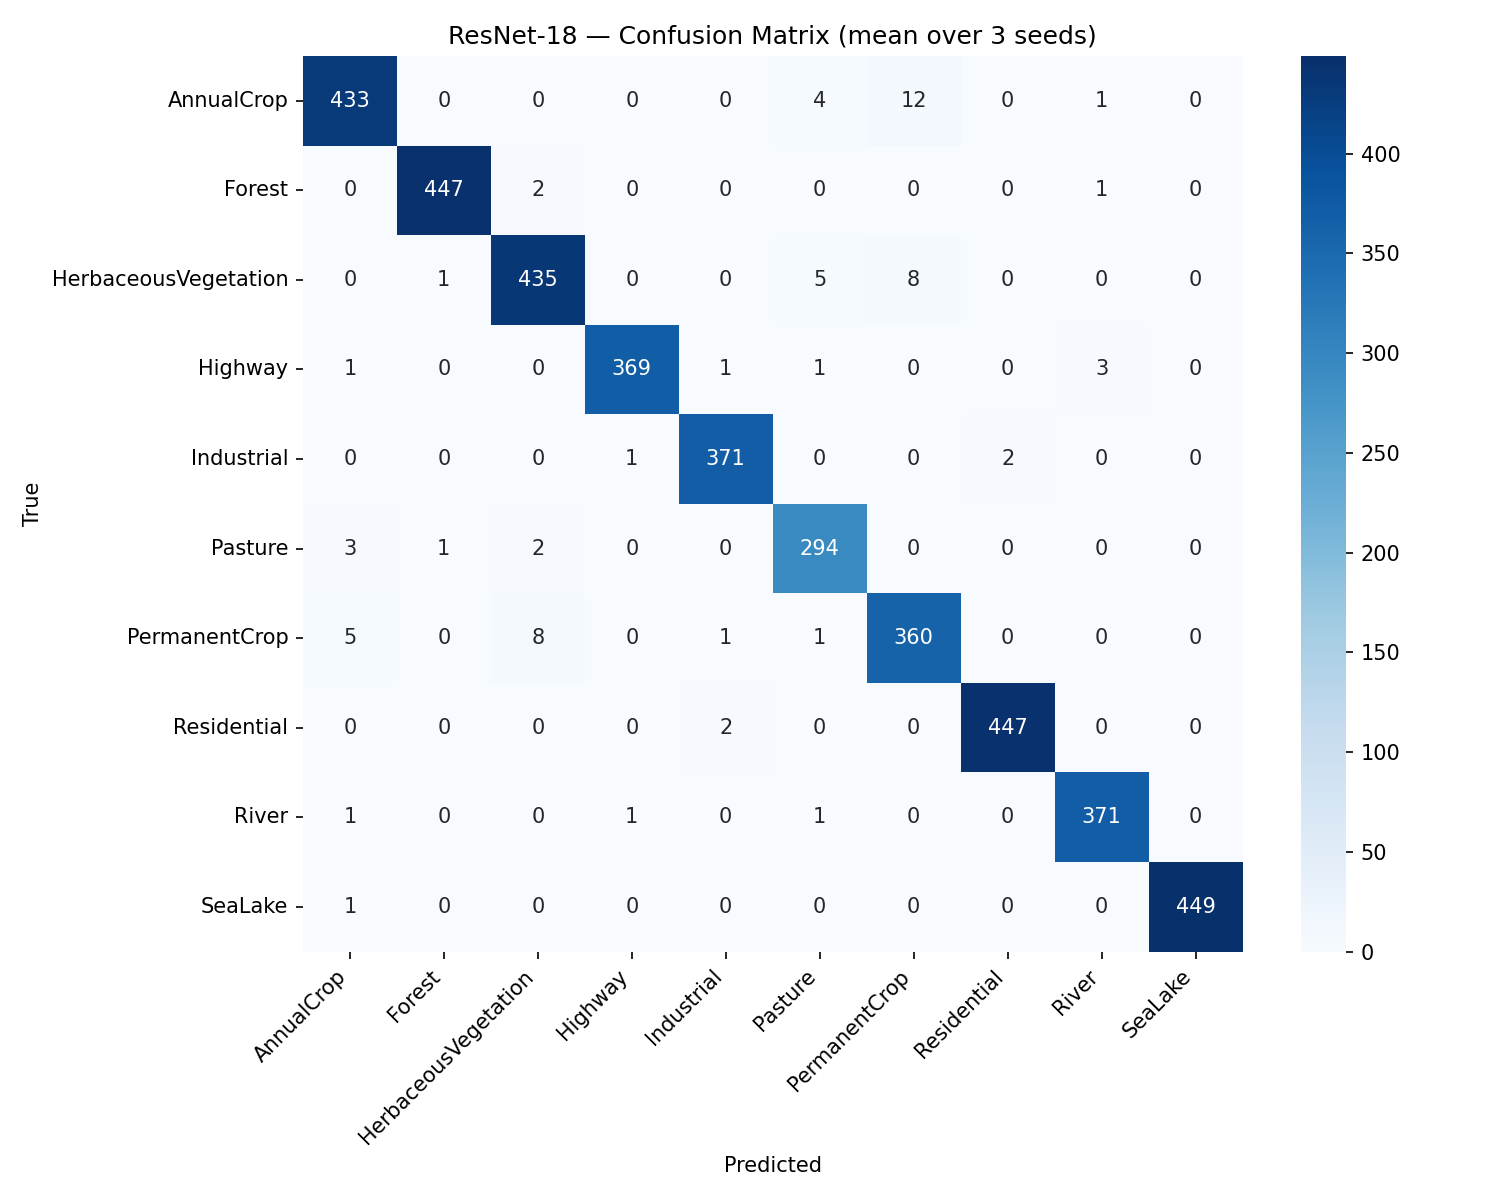
\includegraphics[width=0.65\textwidth]{../results/figures/cm_resnet18_mean.png}
\caption{Tier 4 ResNet-18, confusion matrix averaged over 3 seeds.}
\label{fig:appF-resnet}
\end{figure}

\begin{figure}[h]
\centering
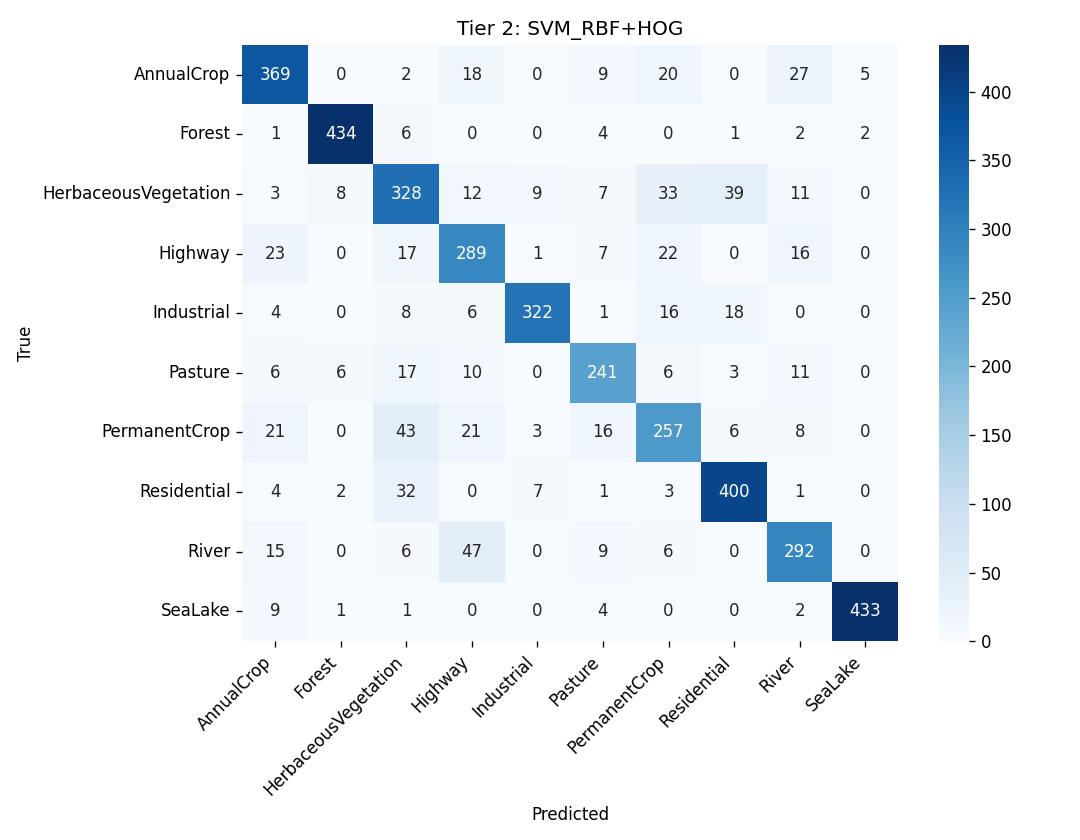
\includegraphics[width=0.65\textwidth]{../results/figures/cm_tier2_SVM_RBF_HOG.png}
\caption{Tier 2 SVM-RBF + HOG, confusion matrix on test set.}
\label{fig:appF-svmhog}
\end{figure}

\begin{figure}[h]
\centering
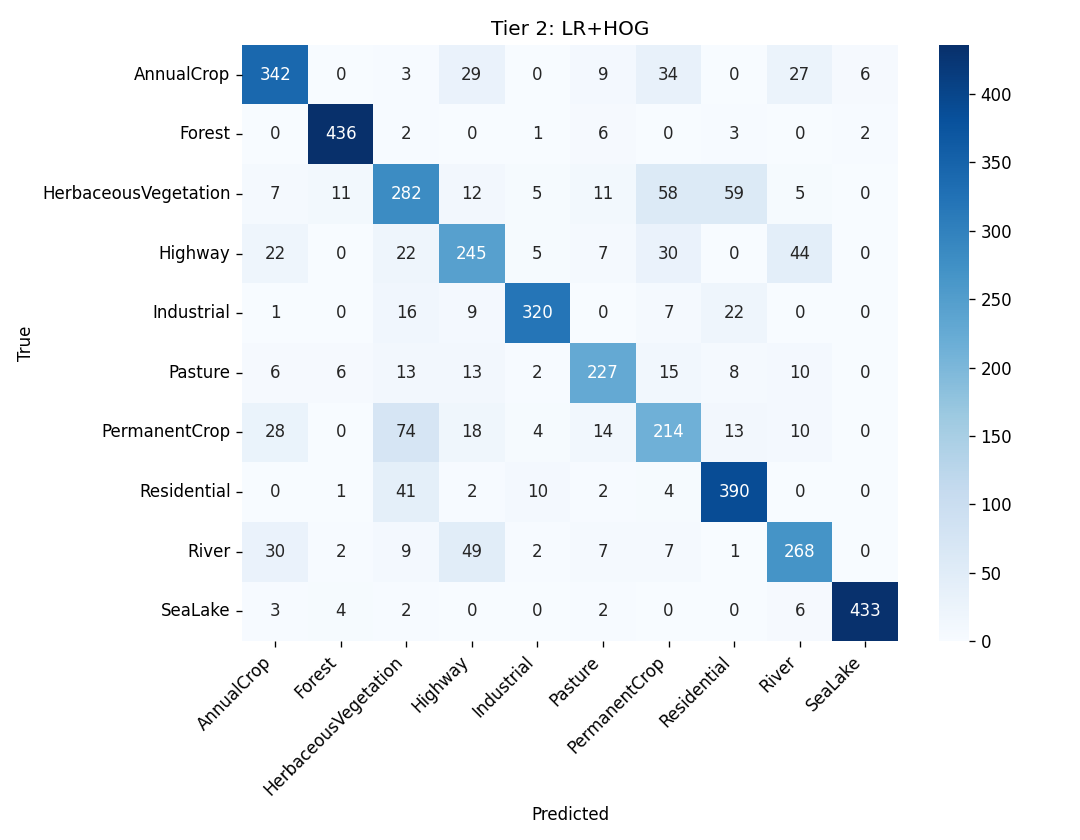
\includegraphics[width=0.65\textwidth]{../results/figures/cm_tier2_LR_HOG.png}
\caption{Tier 2 LR + HOG, confusion matrix on test set.}
\label{fig:appF-lrhog}
\end{figure}
\end{document}